% RESULTADOS Y DISCUSION 

\cleardoublepage

\chapter{Resultados y Discusión}
\label{resultados-y-discusion}

\section{Introducción}
\label{resultados-introduccion}

A continuación haremos un repaso de los resultados obtenidos en el subconjunto de experimentos más representativo, realizados con los diferentes algoritmos propuestos.
\medskip

Detallaremos también las conclusiones parciales que obtenemos en cada experimento, así como posibles soluciones a los problemas que se nos plantean en cada uno.
\medskip

Cabe mencionar que debido al coste computacional de ejecutar cada experimento sobre el conjunto de datos total, cada experimento se compone de subexperimentos previos, en los cuales intentábamos probar nuestras soluciones con un conjunto de datos menor al original, alrededor de unas 20 imágenes. 
\medskip

La idea detrás de esta subexperimentación era conseguir un modelo de agente que sea capaz de realizar overfitting sobre el conjunto de datos de manera relativamente rápida y que obtuviese una convergencia tanto en la recompensa obtenida tanto en las imágenes del conjunto de entrenamiento como en el conjunto de test como en el número de pasos que realizaba sobre cada una de las imágenes. Esto nos permitió también acortar el tiempo entre las diferentes pruebas, lo que provocó que pudiesemos experimentar con diferentes definiciones tanto de nuestra recompensa como de nuestro entorno, así como hacer fine tunning de nuestros hiperparámetros.
\medskip

El total de los experimentos está disponible en el repositorio de \href{https://github.com/lucaswerner90/msc-degree-ai}{GitHub} para un análisis más extenso y se adjunta el título de cada uno de ellos en el Apéndize \ref{apendize-a}. 
\medskip

La herramienta utilizada para monitorear el progreso de las diferentes métricas durante los diferentes entrenamientos es \href{https://www.tensorflow.org/tensorboard?hl=es-419}{Tensorboard}, ya que además de su facil integración con \href{https://pytorch.org/}{PyTorch} nos permitía comparar dichas métricas entre los diferentes experimentos.


\section{Policy Gradient}
\label{resultados-policy-gradient}

Lorem ipsum 
\medskip

\subsection{Experimento 1}
\label{resultados-policy-gradient-experimento-1}

\begin{figure}[H]
	\centering
	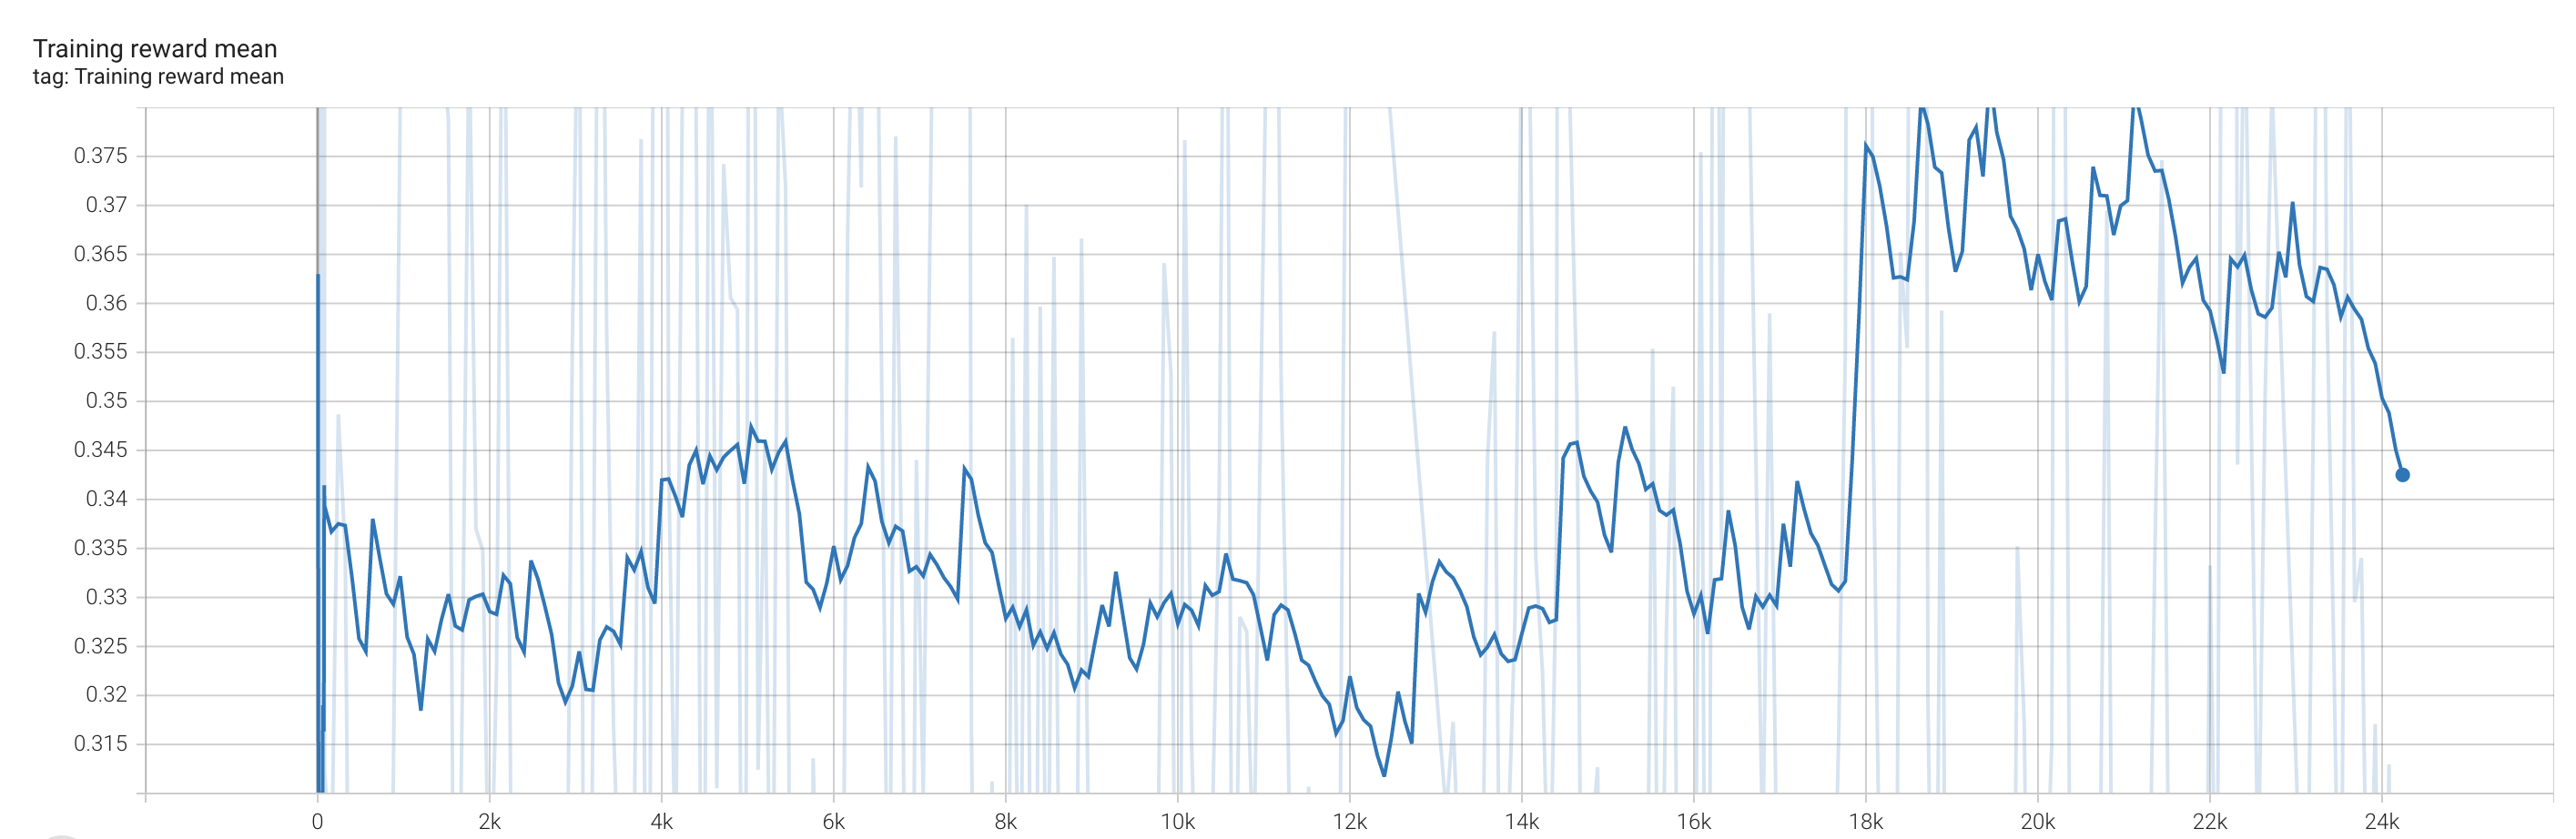
\includegraphics[width=1\textwidth]{figuras/experiments/policy_gradient/policy_gradient_normalized_image_reward_20_epochs/training_reward_mean.png}
	\caption[Experimento Policy Gradient 1 - Training Reward Mean]{Experimento Policy Gradient 1 - Training Reward Mean}
	\label{fig-experimento-policy-gradient-1-training-reward-mean}
\end{figure}

\begin{figure}[H]
	\centering
	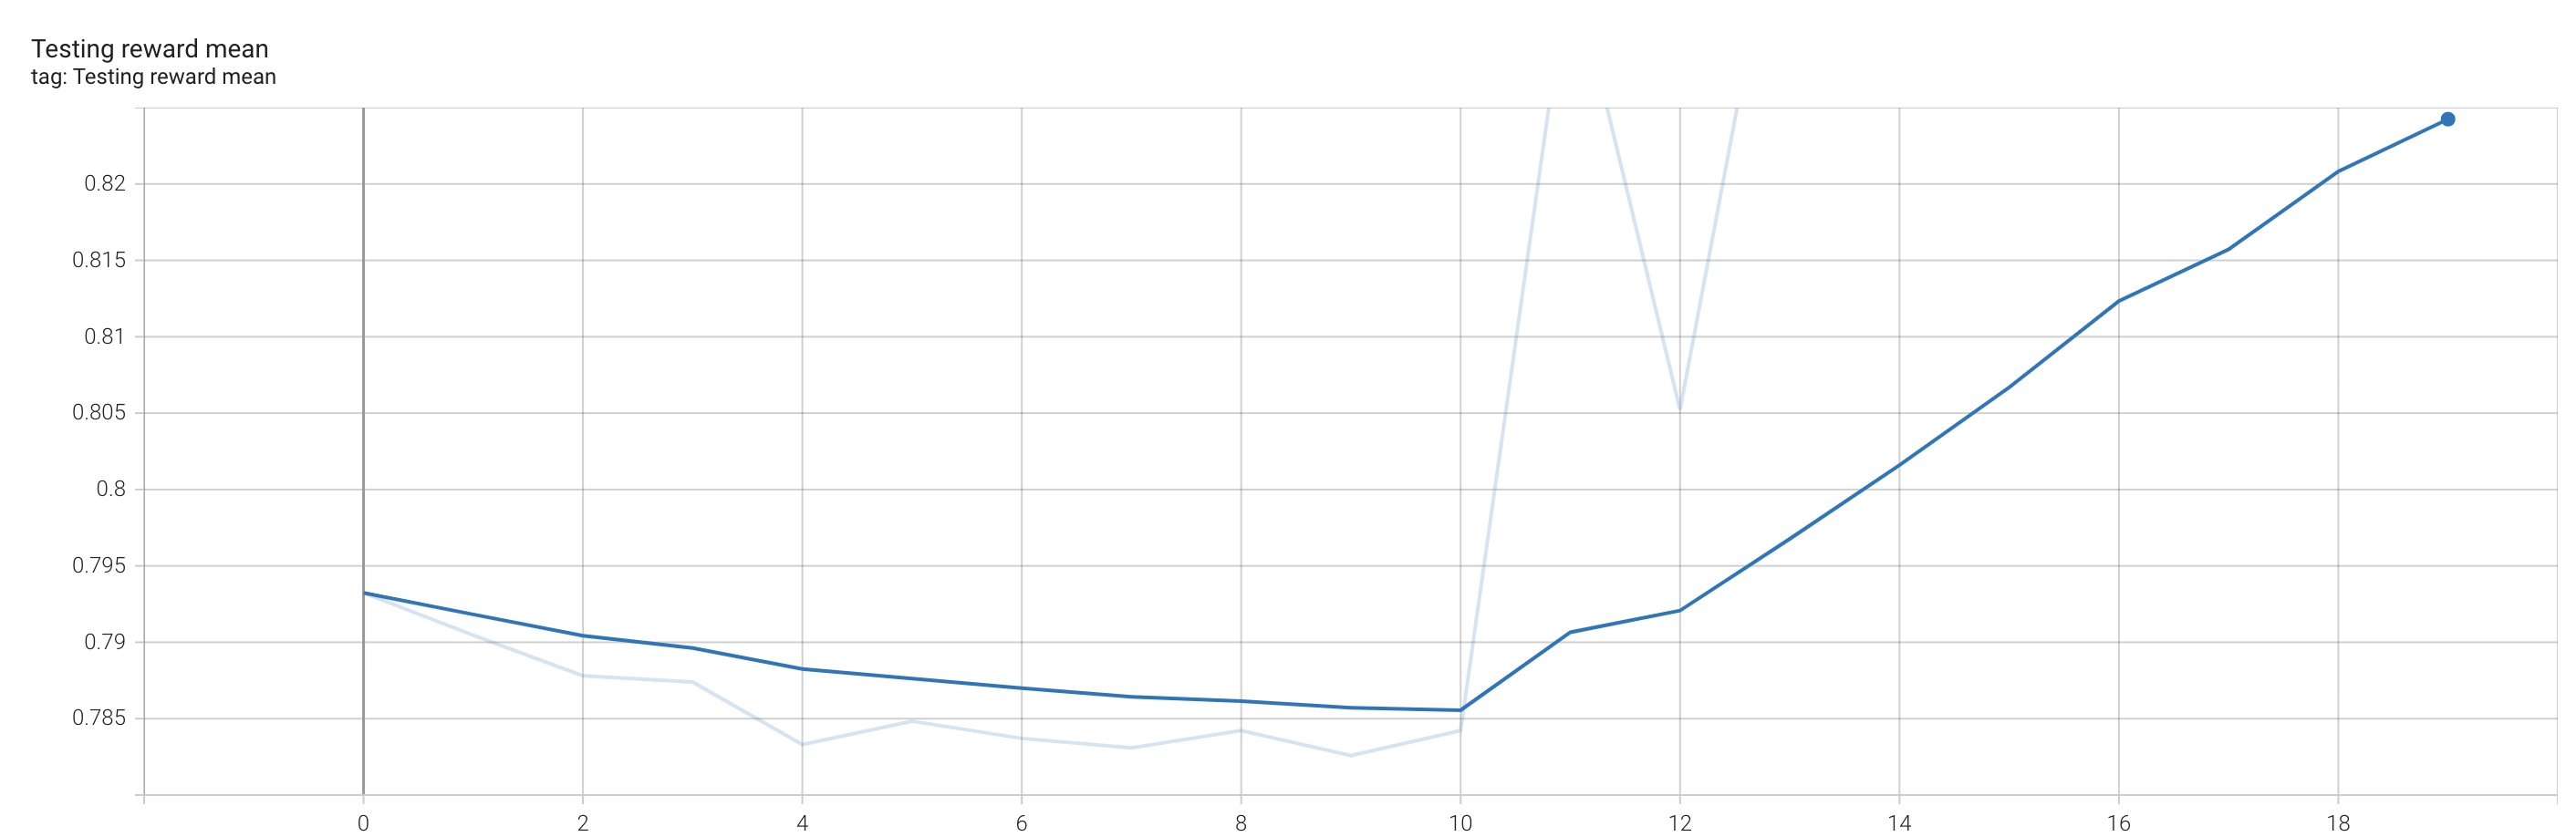
\includegraphics[width=1\textwidth]{figuras/experiments/policy_gradient/policy_gradient_normalized_image_reward_20_epochs/testing_reward_mean.png}
	\caption[Experimento Policy Gradient 1 - Testing reward mean]{Experimento Policy Gradient 1 - Testing reward mean}
	\label{fig-experimento-policy-gradient-1-testing-reward-mean}
\end{figure}
\begin{figure}[H]
	\centering
	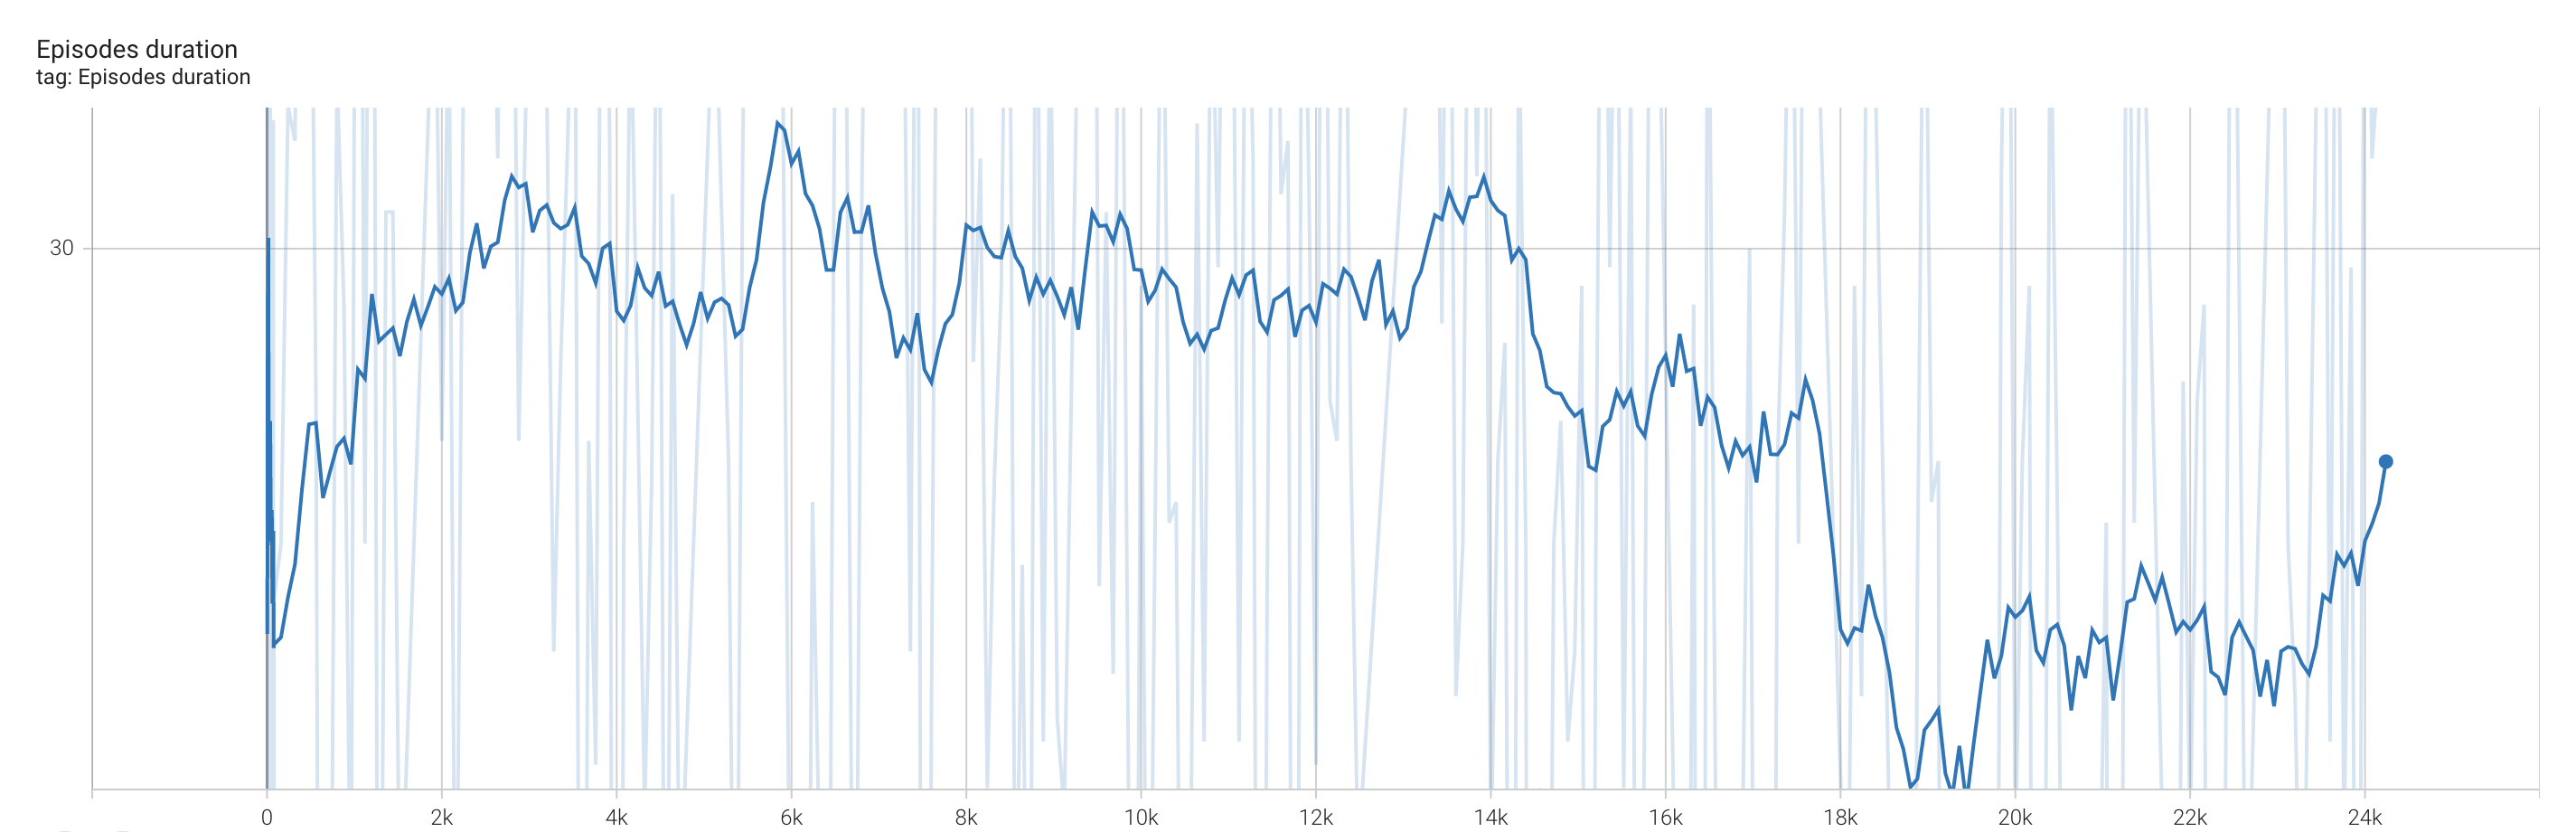
\includegraphics[width=1\textwidth]{figuras/experiments/policy_gradient/policy_gradient_normalized_image_reward_20_epochs/episodes_duration.png}
	\caption[Experimento Policy Gradient 1 - Episodes duration]{Experimento Policy Gradient 1 - Episodes duration}
	\label{fig-experimento-policy-gradient-1-episodes-duration}
\end{figure}

\subsection{Experimento 2}
\label{resultados-policy-gradient-experimento-2}

Los resultados de este experimento son similares al anterior, pero en este caso el entrenamiento se ejecuta durante unas 50 épocas, unas 30 más que el experimento \ref{resultados-policy-gradient-experimento-1}.

\begin{figure}[H]
	\centering
	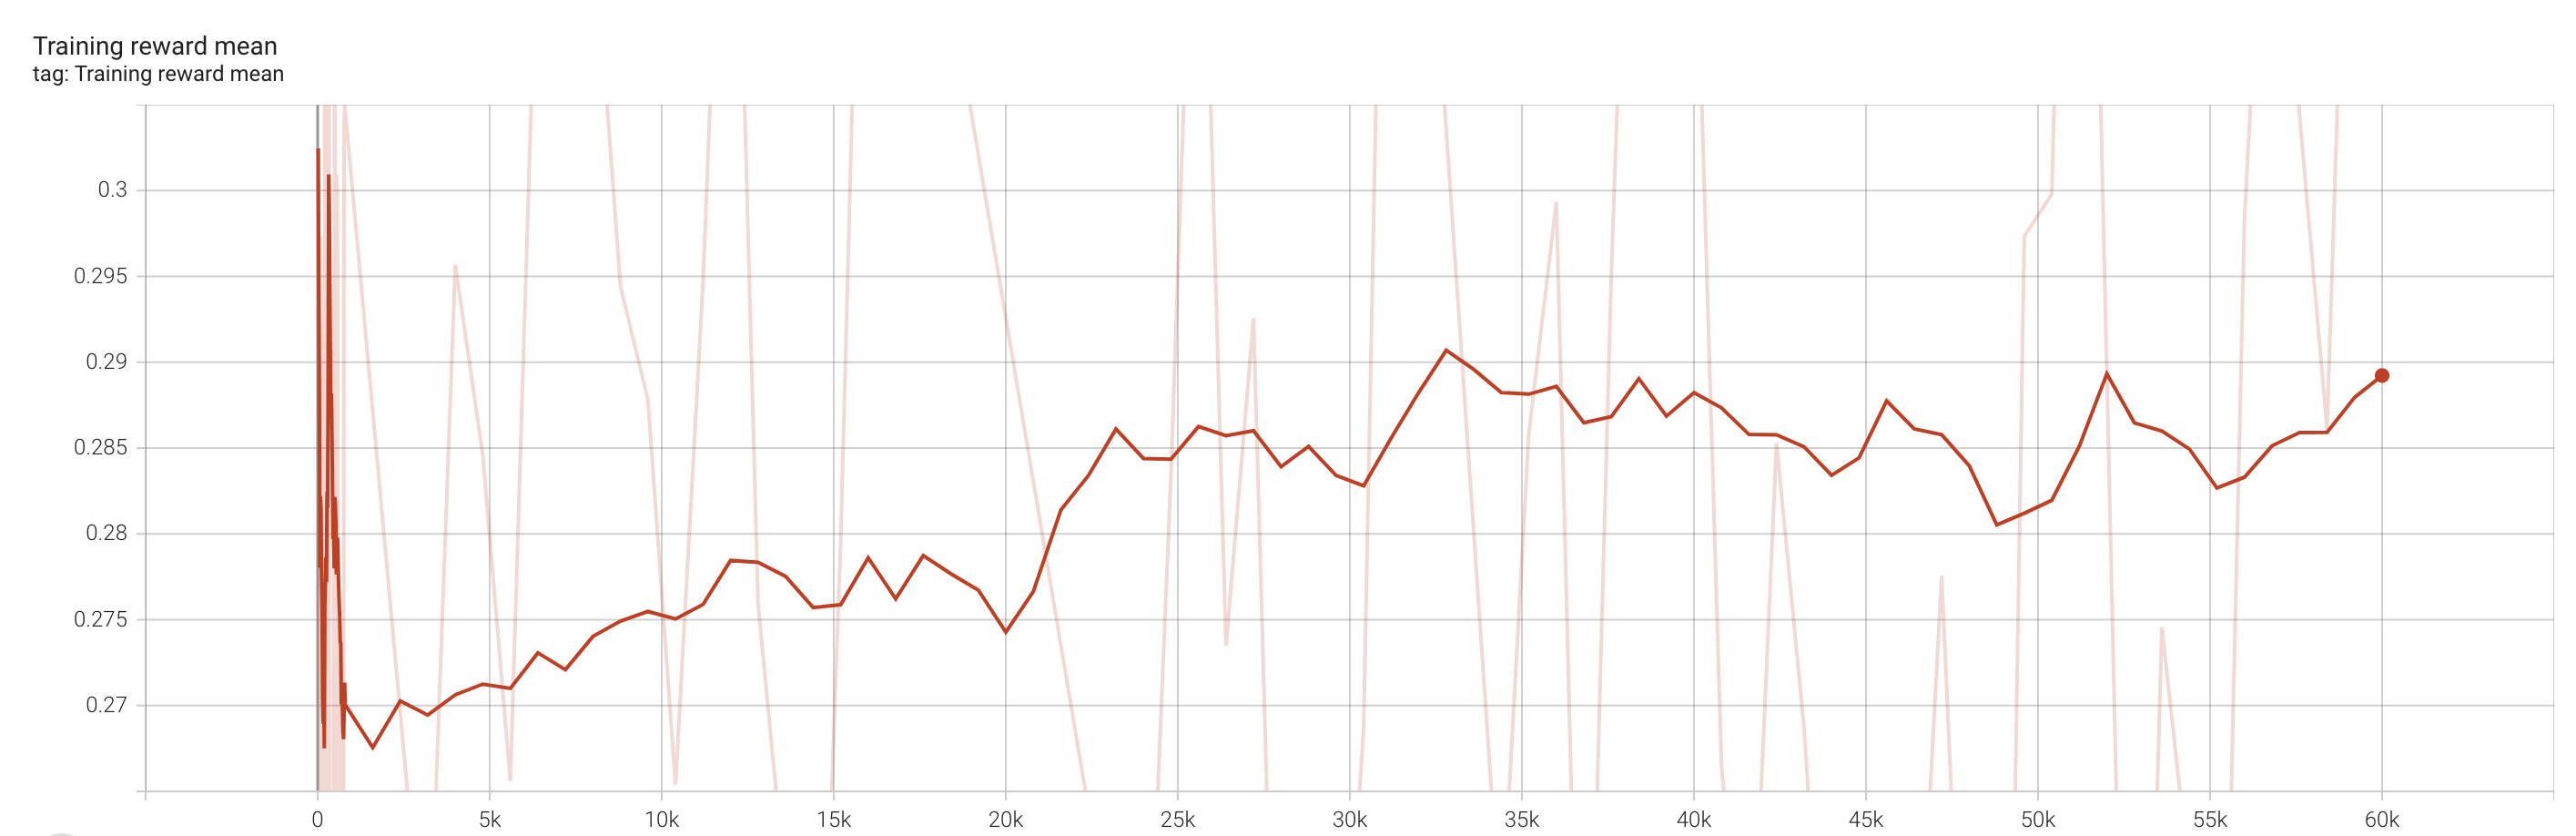
\includegraphics[width=1\textwidth]{figuras/experiments/policy_gradient/policy_gradient_normalized_image_reward_50_epochs/training_reward_mean.png}
	\caption[Experimento Policy Gradient 2 - Training Reward Mean]{Experimento Policy Gradient 2 - Training Reward Mean}
	\label{fig-experimento-policy-gradient-2-training-reward-mean}
\end{figure}
\begin{figure}[H]
	\centering
	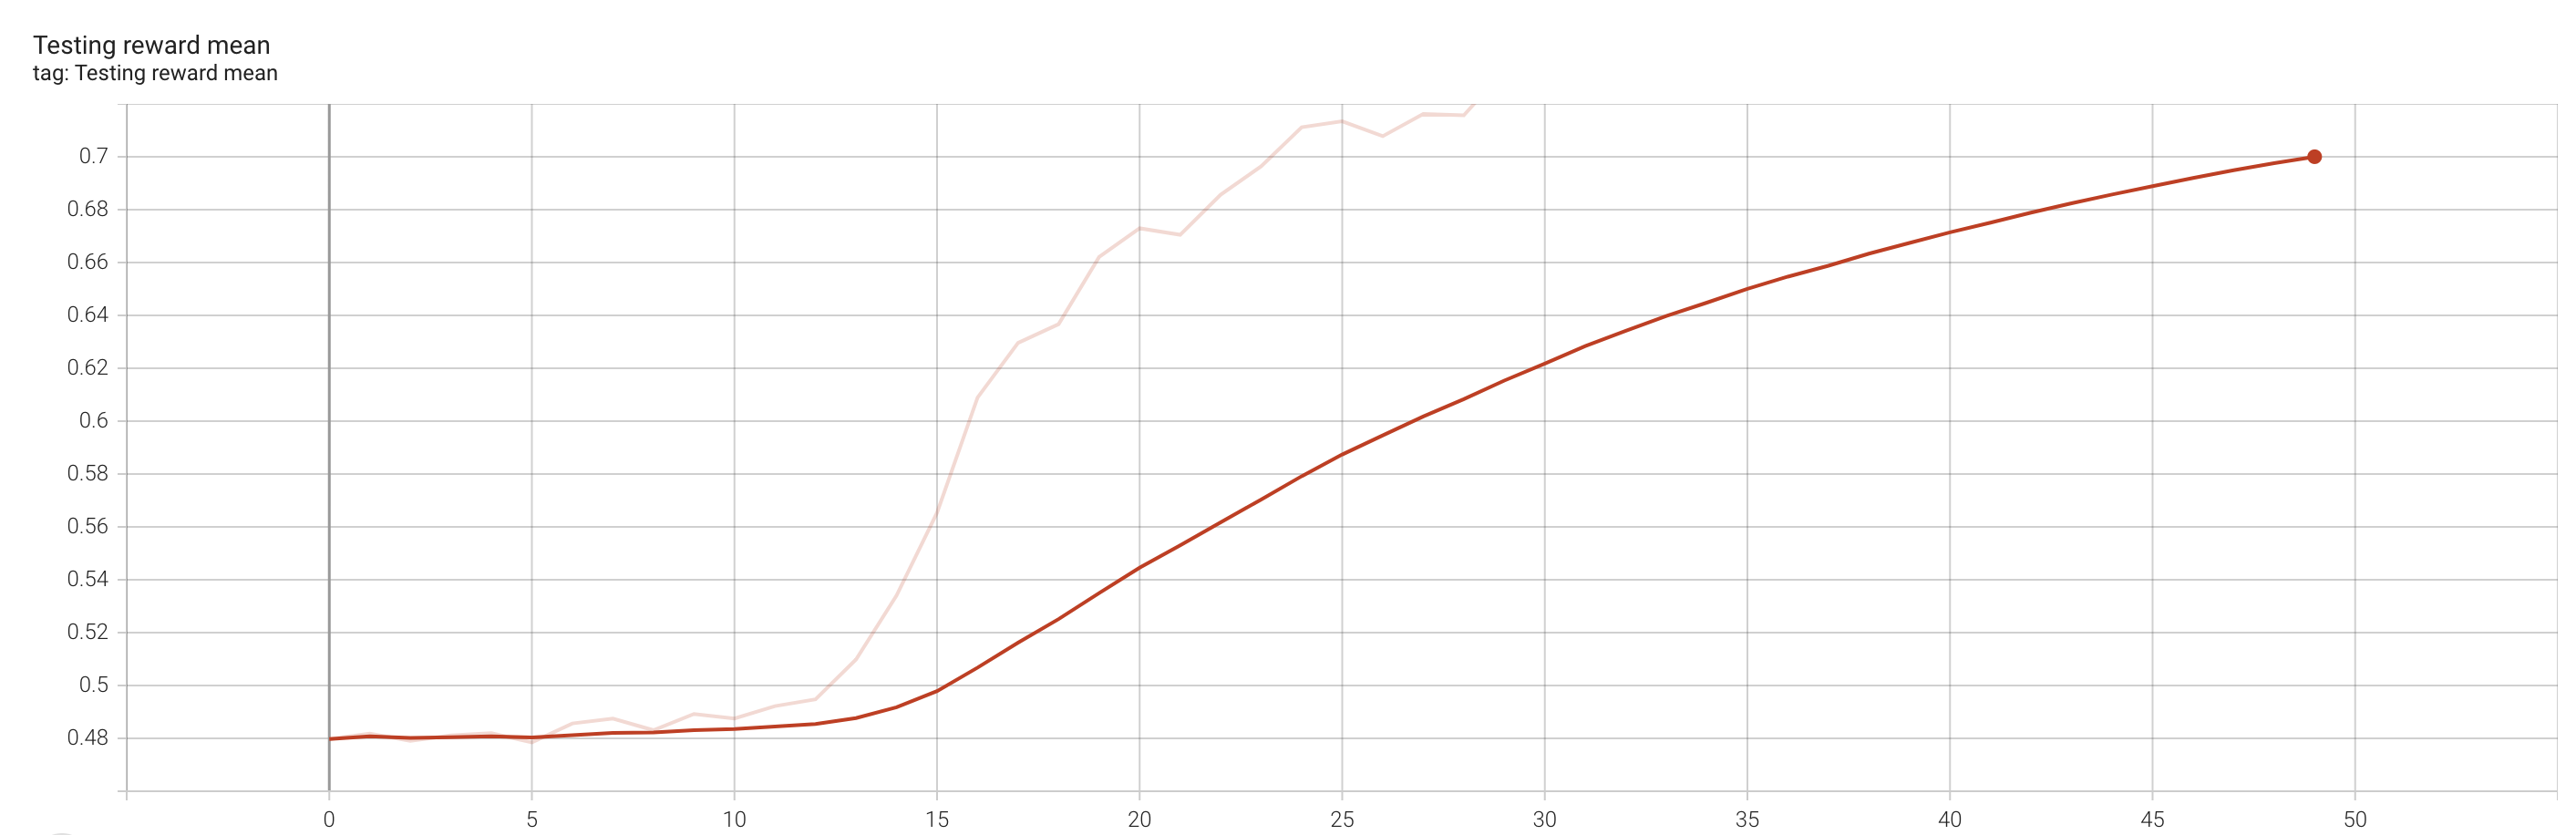
\includegraphics[width=1\textwidth]{figuras/experiments/policy_gradient/policy_gradient_normalized_image_reward_50_epochs/testing_reward_mean.png}
	\caption[Experimento Policy Gradient 2 - Testing reward mean]{Experimento Policy Gradient 2 - Testing reward mean}
	\label{fig-experimento-policy-gradient-2-testing-reward-mean}
\end{figure}
\begin{figure}[H]
	\centering
	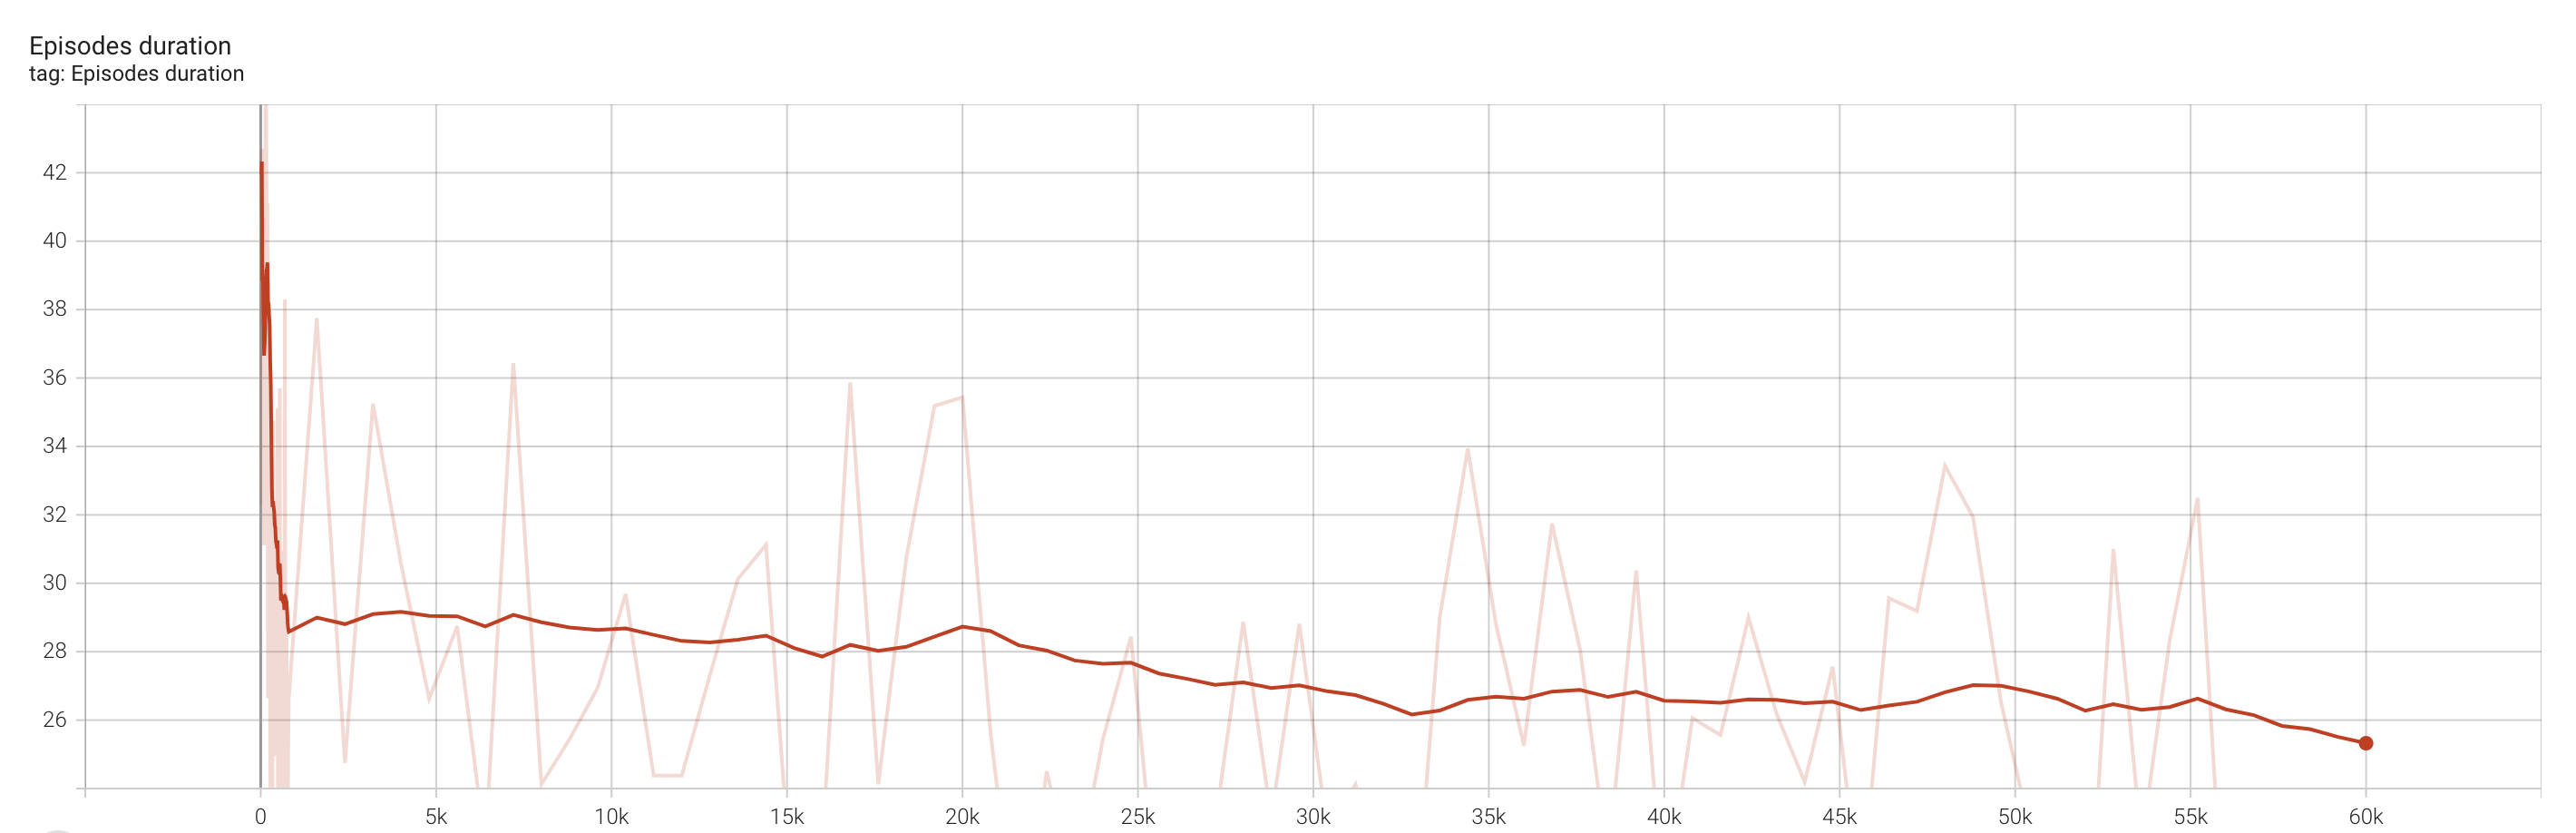
\includegraphics[width=1\textwidth]{figuras/experiments/policy_gradient/policy_gradient_normalized_image_reward_50_epochs/episodes_duration.png}
	\caption[Experimento Policy Gradient 2 - Episodes duration]{Experimento Policy Gradient 2 - Episodes duration}
	\label{fig-experimento-policy-gradient-2-episodes-duration}
\end{figure}

\section{Actor-Critic}
\label{resultados-actor-critic}

Veremos ahora el comportamiento de algunos de los experimentos llevados a cabo con el algoritmo Actor Critic.
\medskip

\subsection{Experimento 1}
\label{resultados-actor-critic-experimento-1}

\begin{figure}[H]
	\centering
	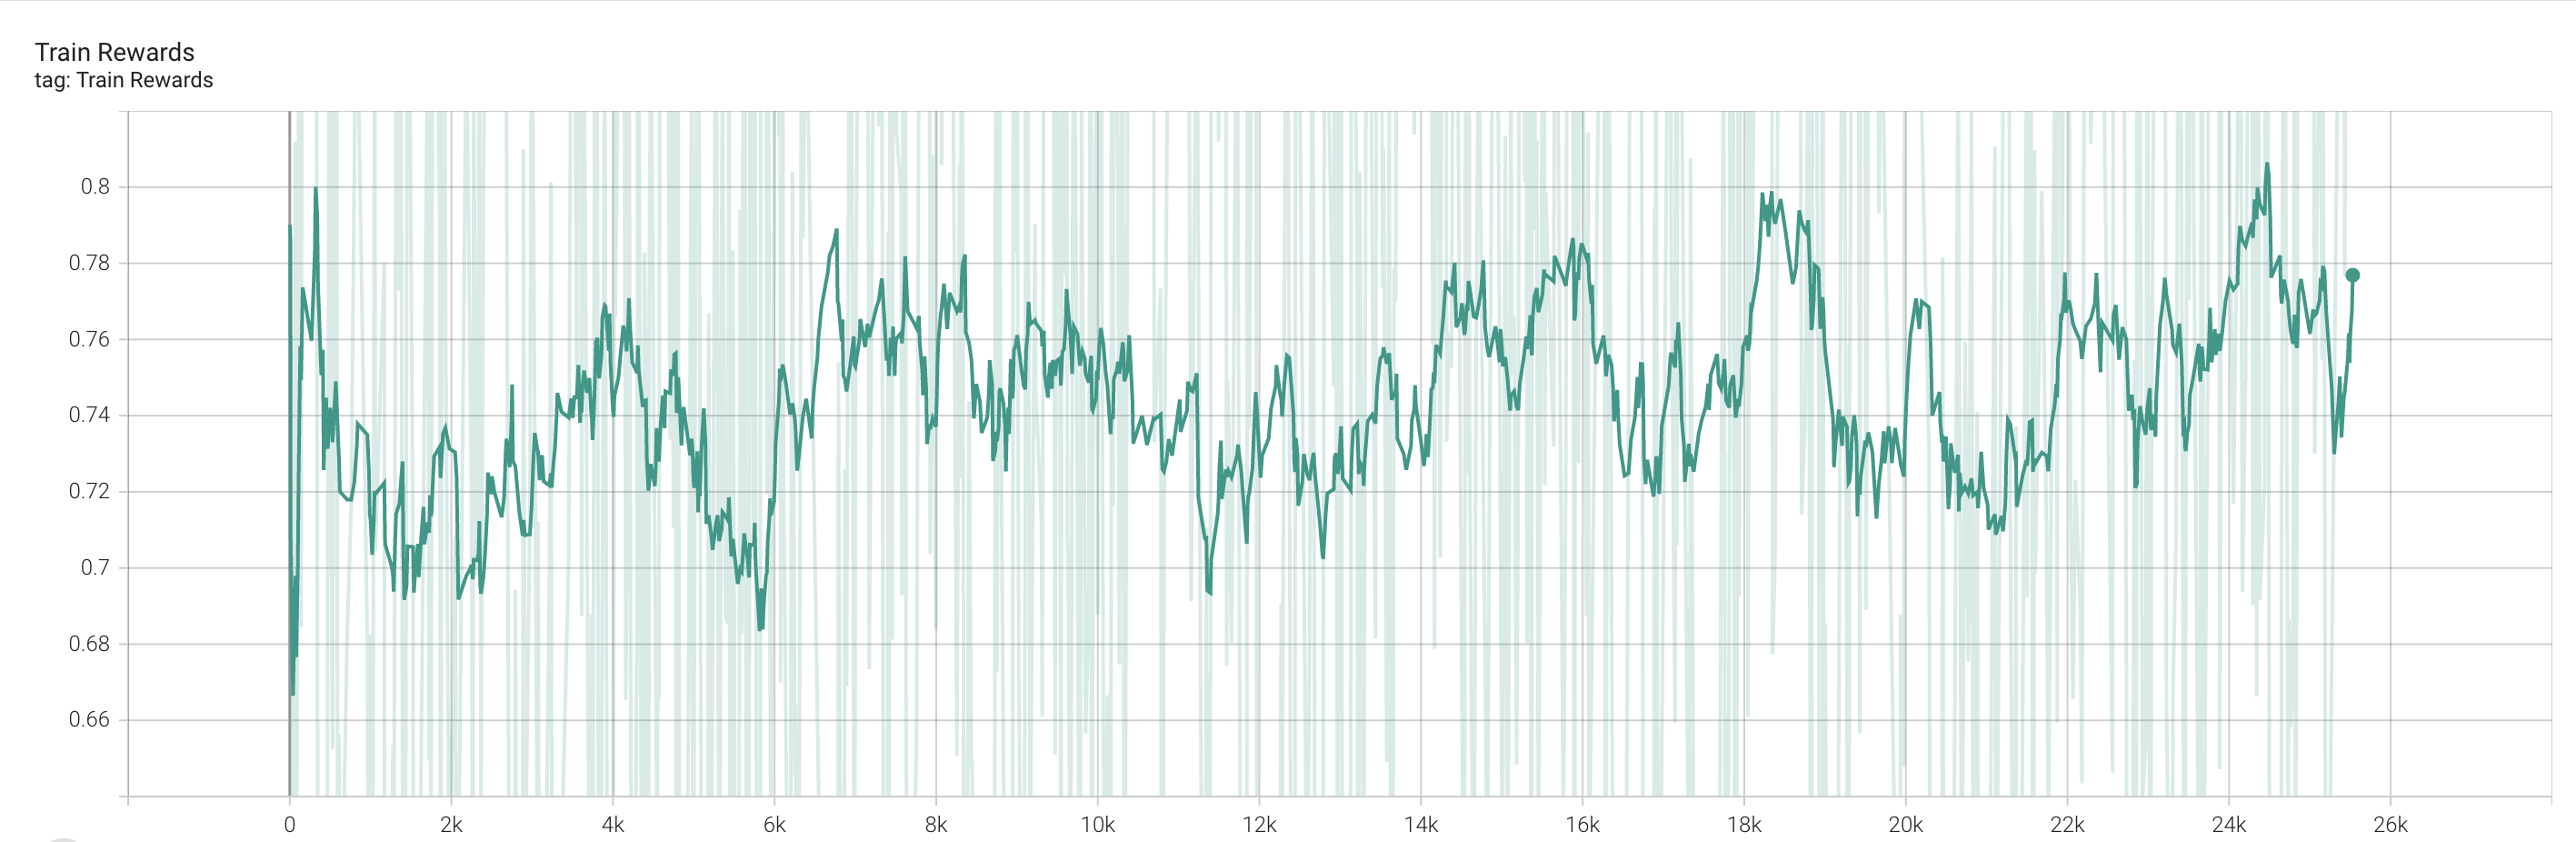
\includegraphics[width=1\textwidth]{figuras/experiments/actor_critic/actor_critic_20_epochs/train_rewards.png}
	\caption[Experimento Actor Critic 1 - Training Reward Mean]{Experimento Actor Critic 1 - Training Reward Mean}
	\label{fig-experimento-actor-critic-1-training-reward-mean}
\end{figure}
\begin{figure}[H]
	\centering
	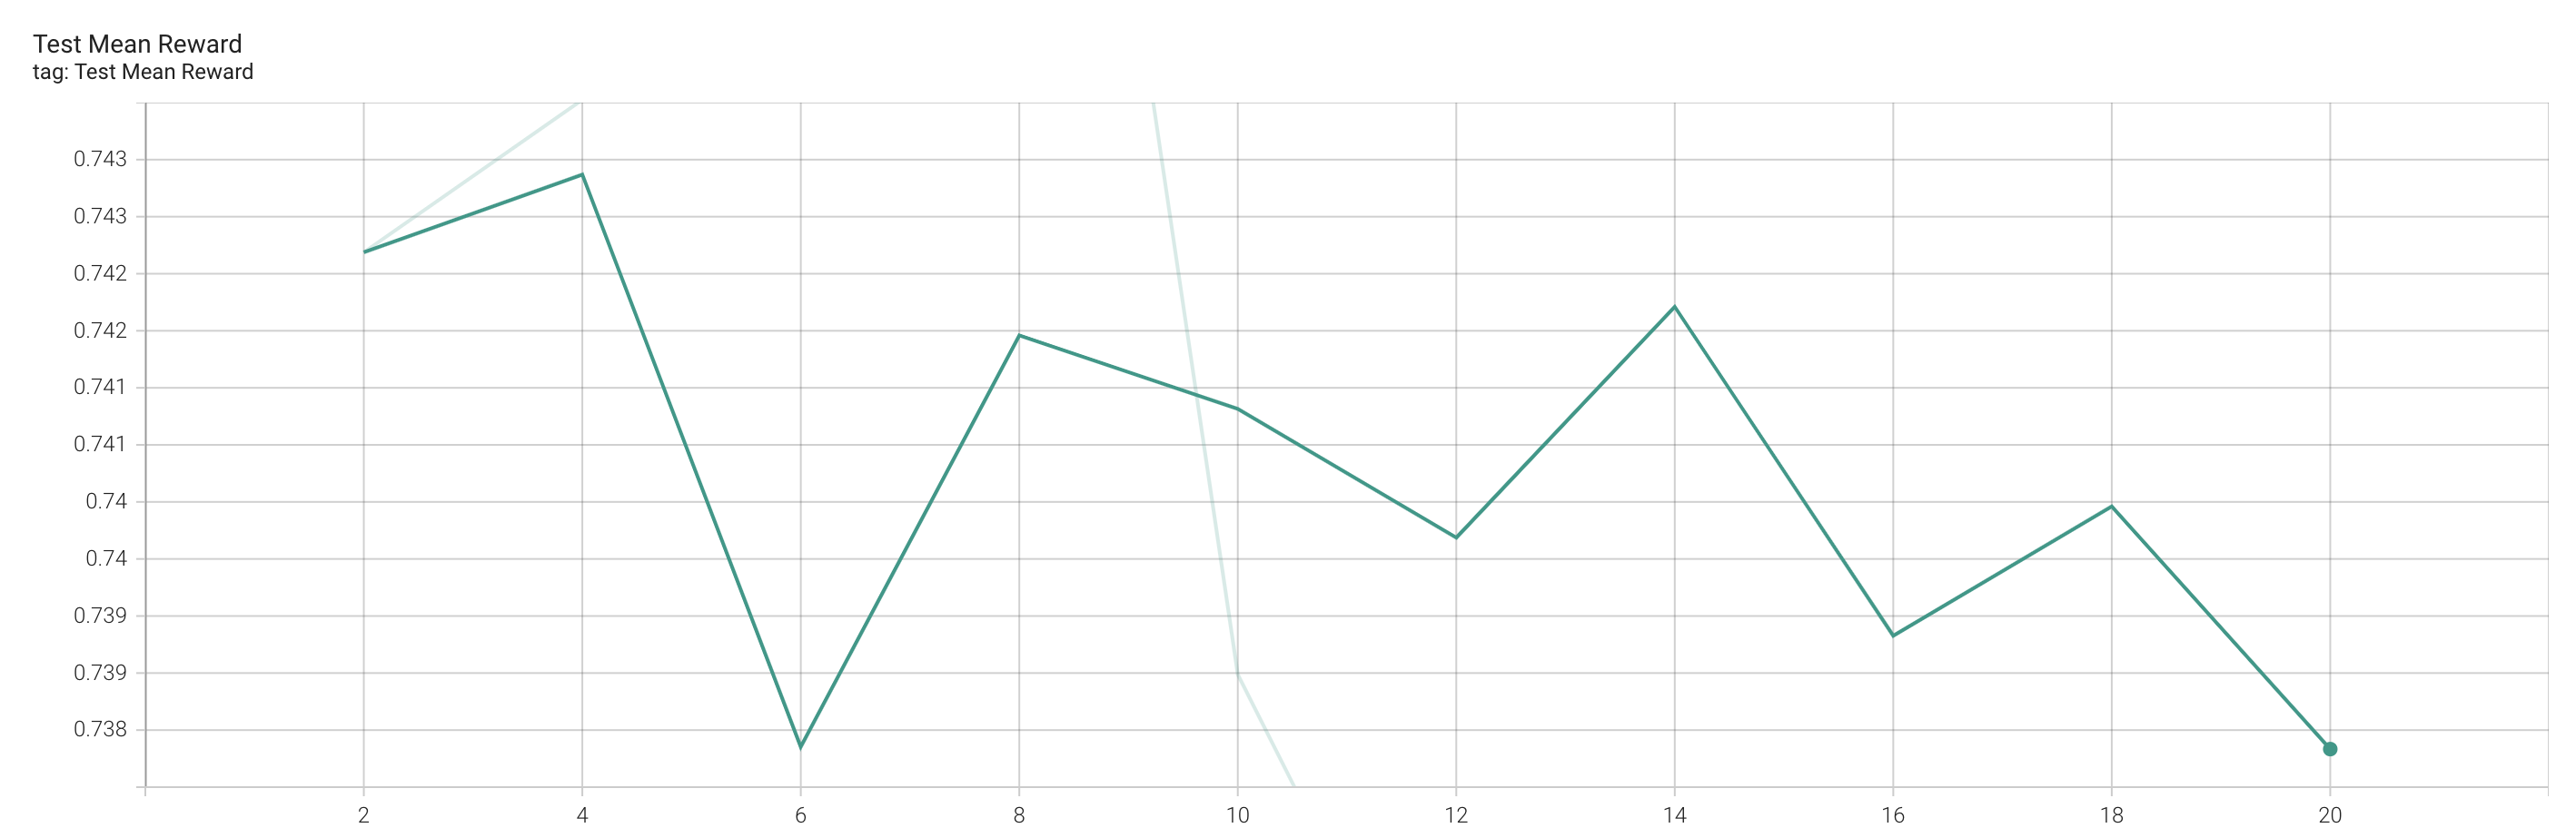
\includegraphics[width=1\textwidth]{figuras/experiments/actor_critic/actor_critic_20_epochs/test_mean_reward.png}
	\caption[Experimento Actor Critic 1 - Testing reward mean]{Experimento Actor Critic 1 - Testing reward mean}
	\label{fig-experimento-actor-critic-1-testing-reward-mean}
\end{figure}
\begin{figure}[H]
	\centering
	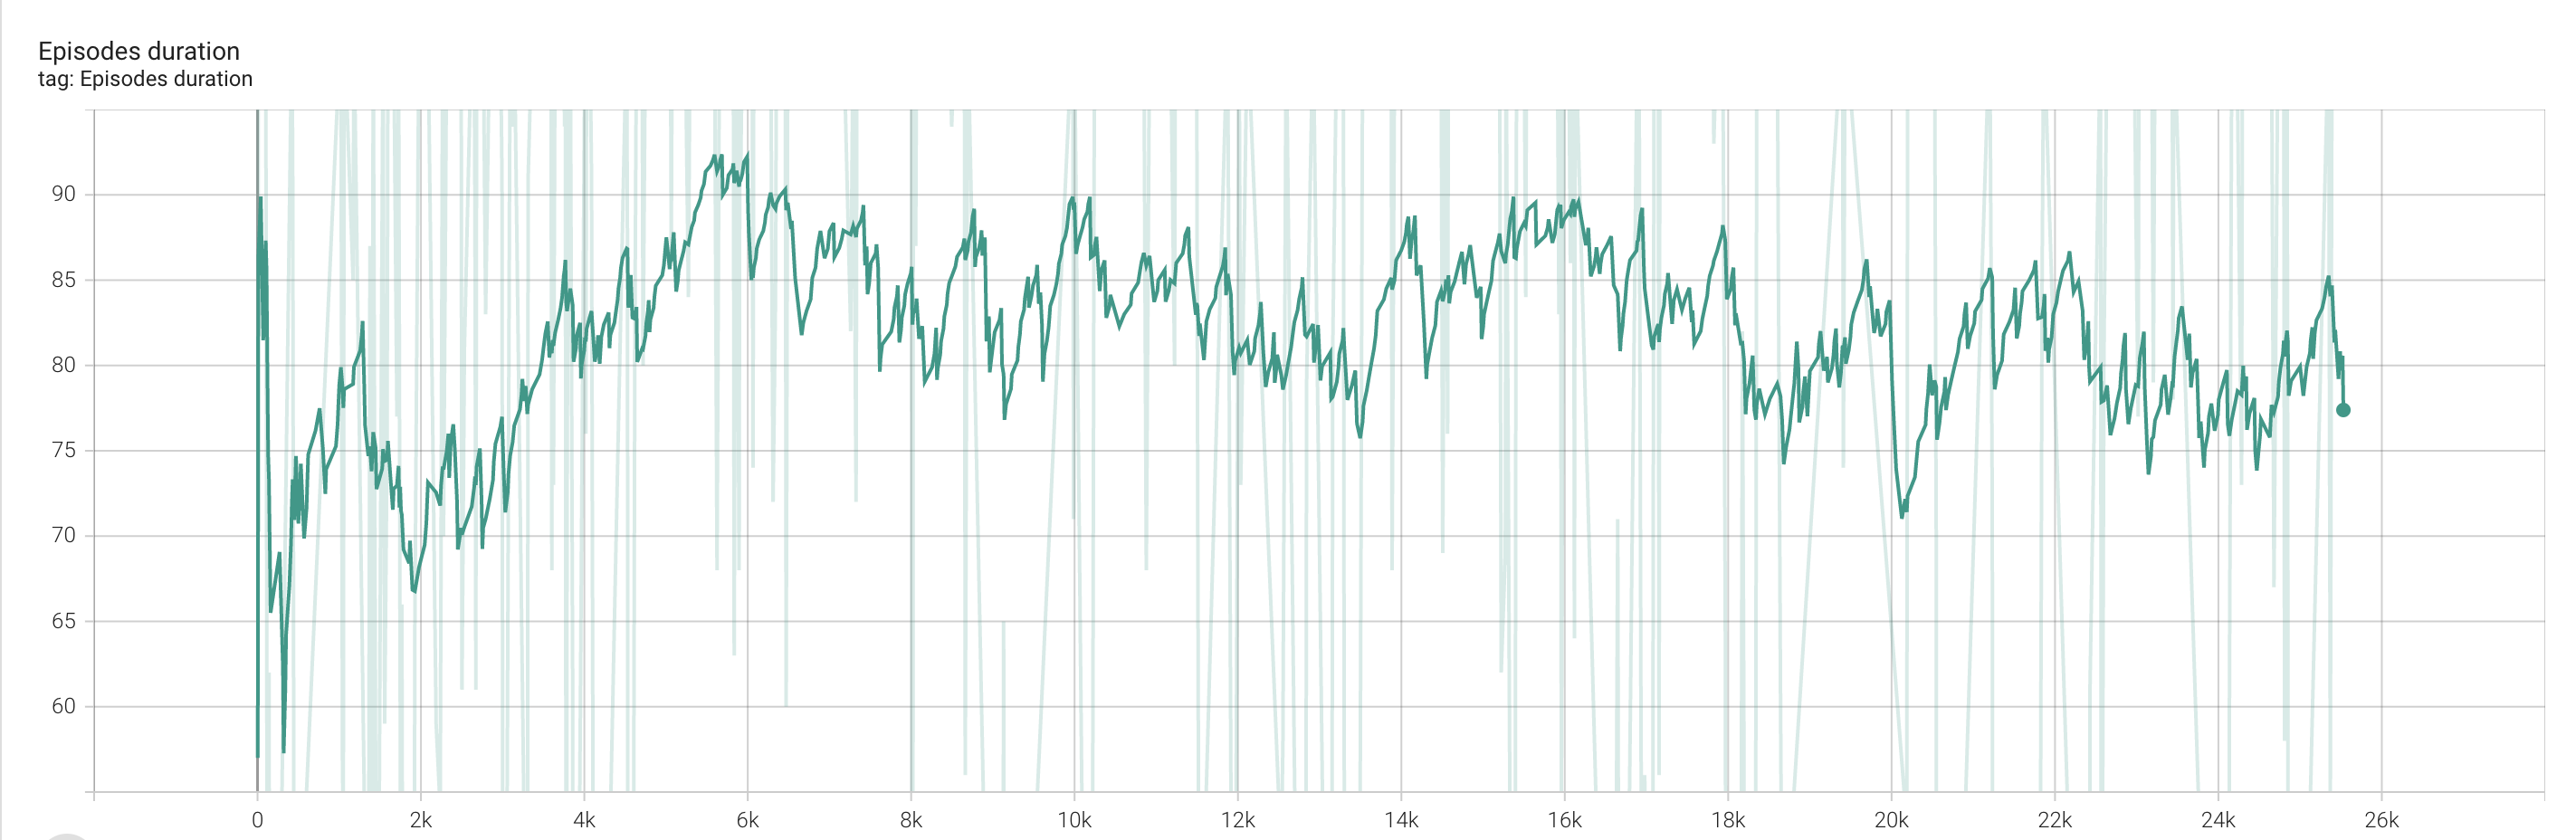
\includegraphics[width=1\textwidth]{figuras/experiments/actor_critic/actor_critic_20_epochs/episodes_duration.png}
	\caption[Experimento Actor Critic 1 - Episodes duration]{Experimento Actor Critic 1 - Episodes duration}
	\label{fig-experimento-actor-critic-1-episodes-duration}
\end{figure}

\subsection{Experimento 2}
\label{resultados-actor-critic-experimento-2}

\begin{figure}[H]
	\centering
	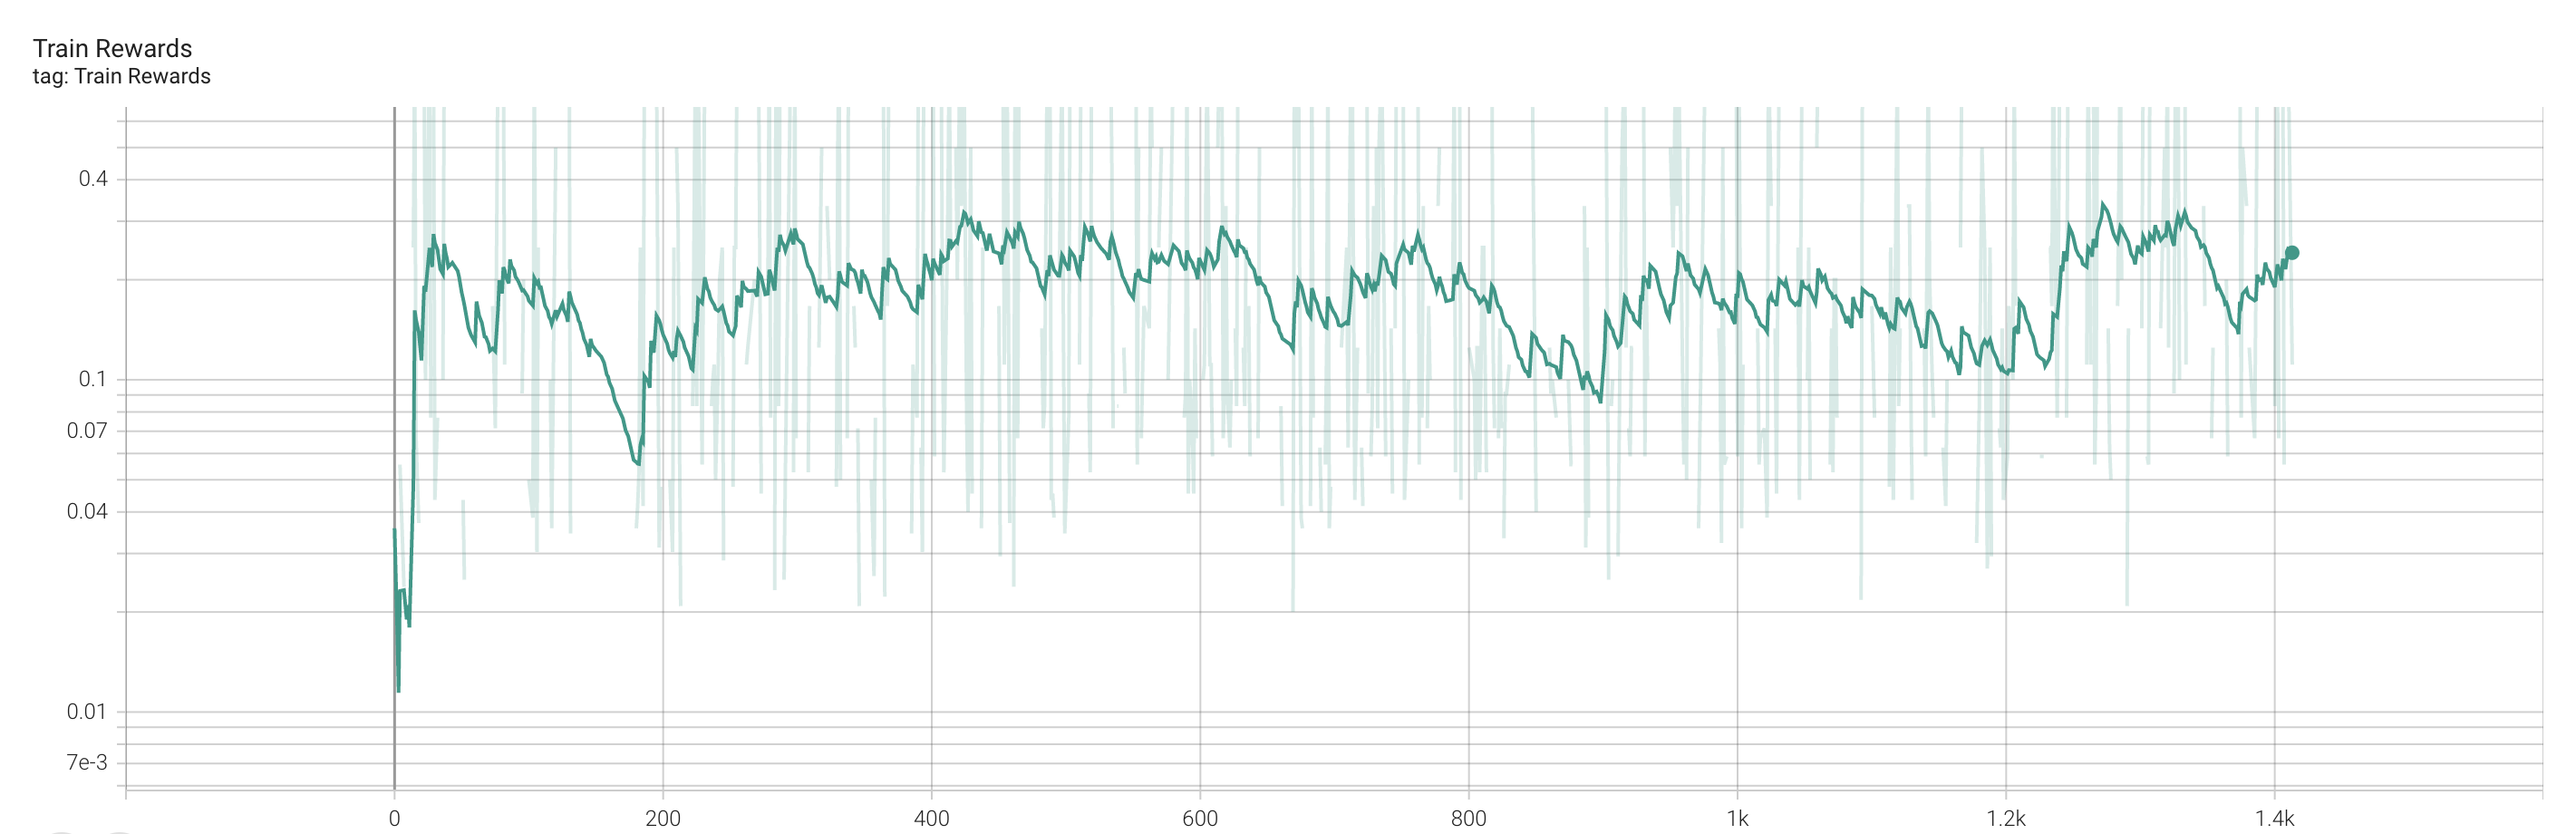
\includegraphics[width=1\textwidth]{figuras/experiments/actor_critic/actor_critic_no_rewards_till_complete/train_rewards.png}
	\caption[Experimento Actor Critic 2 - Training Reward Mean]{Experimento Actor Critic 2 - Training Reward Mean}
	\label{fig-experimento-actor-critic-2-training-reward-mean}
\end{figure}
\begin{figure}[H]
	\centering
	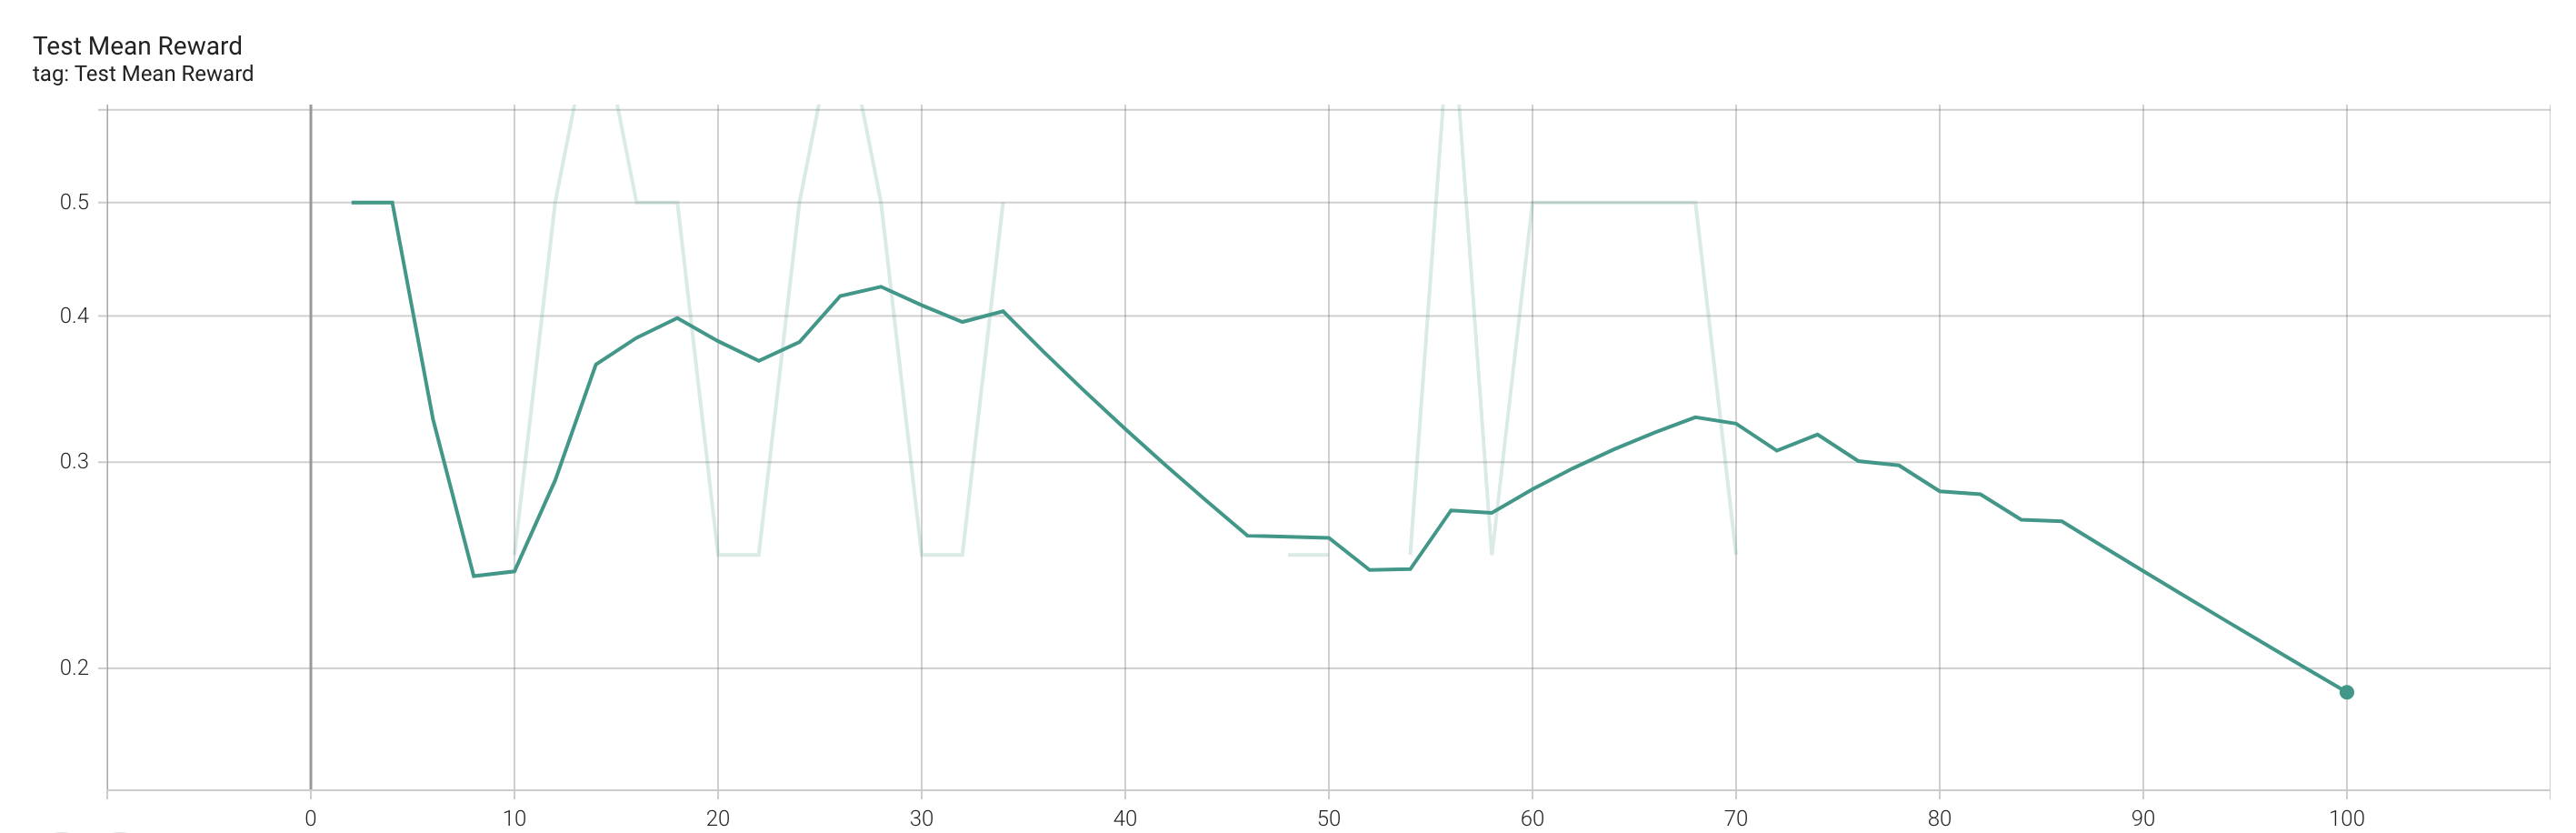
\includegraphics[width=1\textwidth]{figuras/experiments/actor_critic/actor_critic_no_rewards_till_complete/test_mean_reward.png}
	\caption[Experimento Actor Critic 2 - Testing reward mean]{Experimento Actor Critic 2 - Testing reward mean}
	\label{fig-experimento-actor-critic-2-testing-reward-mean}
\end{figure}
\begin{figure}[H]
	\centering
	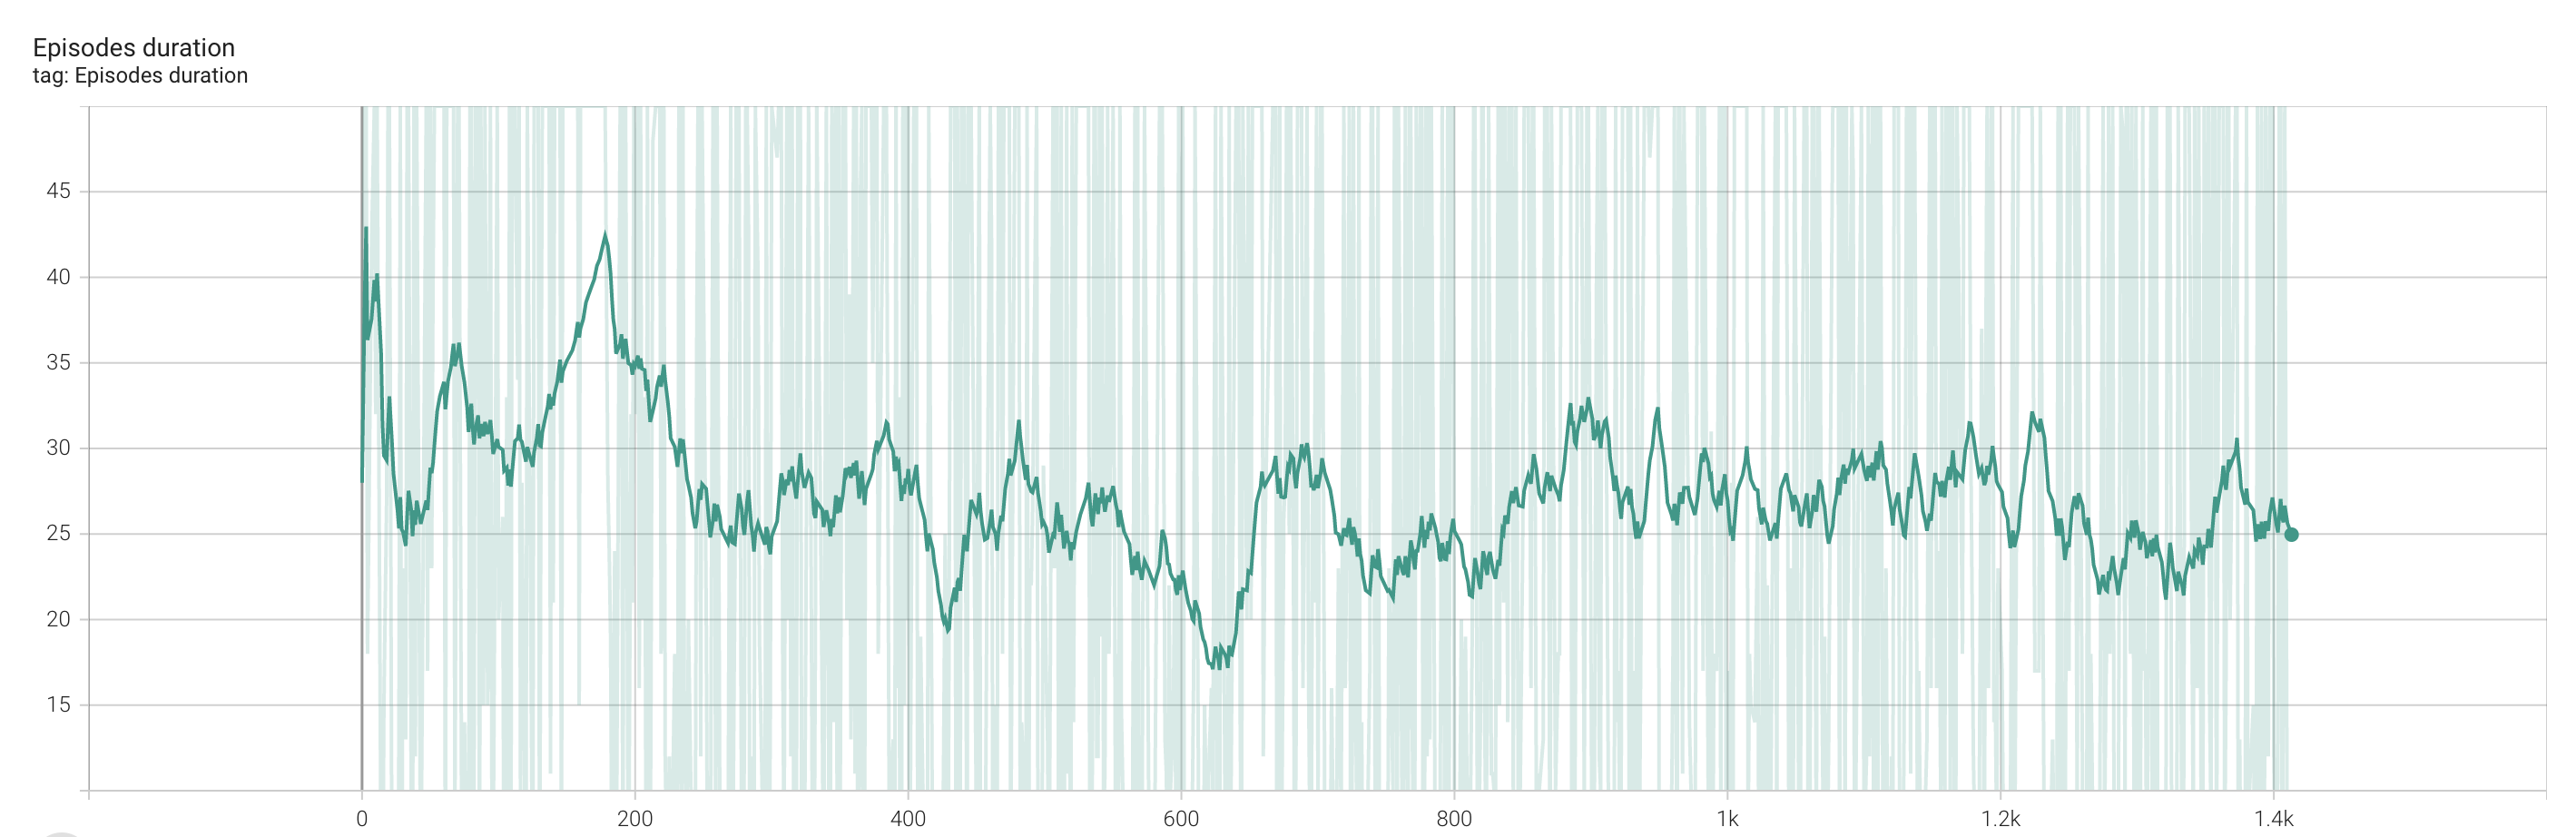
\includegraphics[width=1\textwidth]{figuras/experiments/actor_critic/actor_critic_no_rewards_till_complete/episodes_duration.png}
	\caption[Experimento Actor Critic 2 - Episodes duration]{Experimento Actor Critic 2 - Episodes duration}
	\label{fig-experimento-actor-critic-2-episodes-duration}
\end{figure}

\subsection{Experimento 3}
\label{resultados-actor-critic-experimento-3}


\begin{figure}[H]
	\centering
	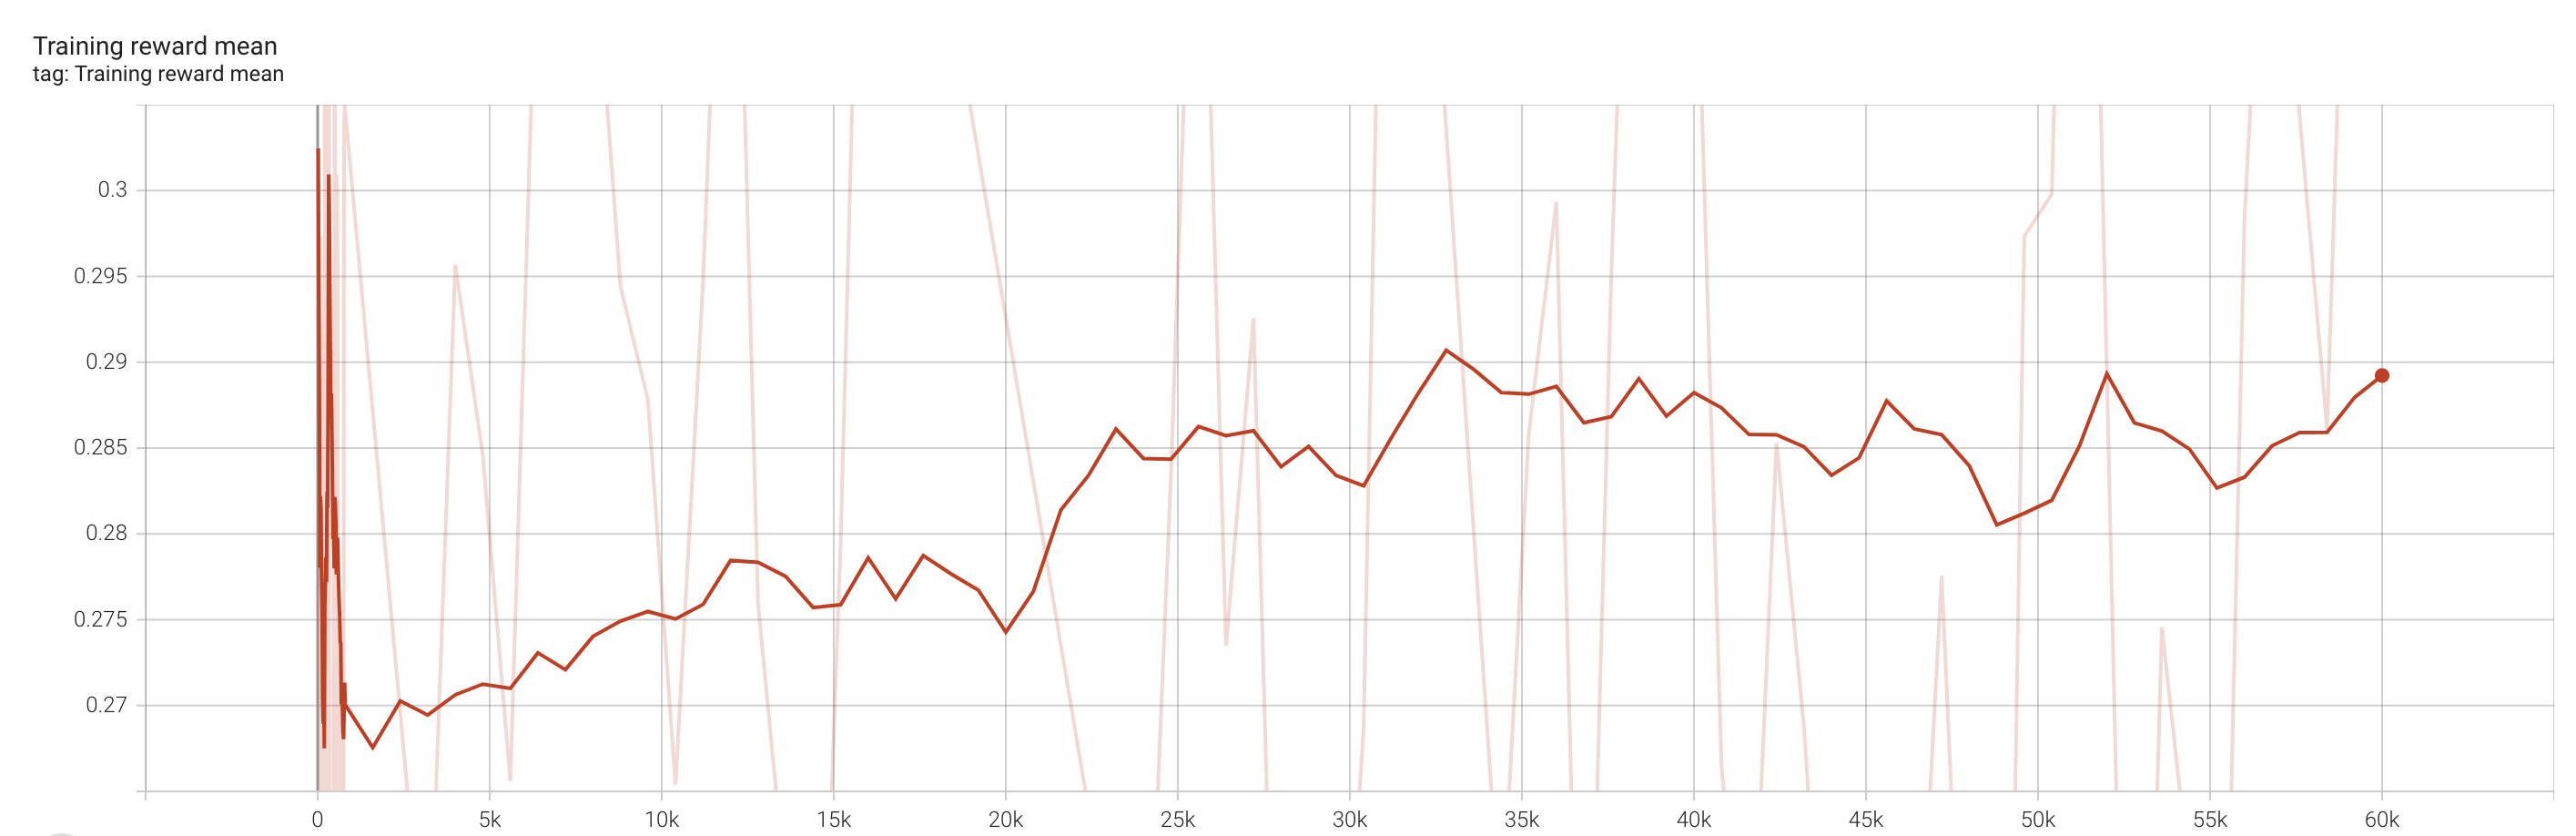
\includegraphics[width=1\textwidth]{figuras/experiments/policy_gradient/policy_gradient_normalized_image_reward_50_epochs/training_reward_mean.png}
	\caption[Experimento Actor Critic 3 - Training Reward Mean]{Experimento Actor Critic 3 - Training Reward Mean}
	\label{fig-experimento-actor-critic-3-training-reward-mean}
\end{figure}
\begin{figure}[H]
	\centering
	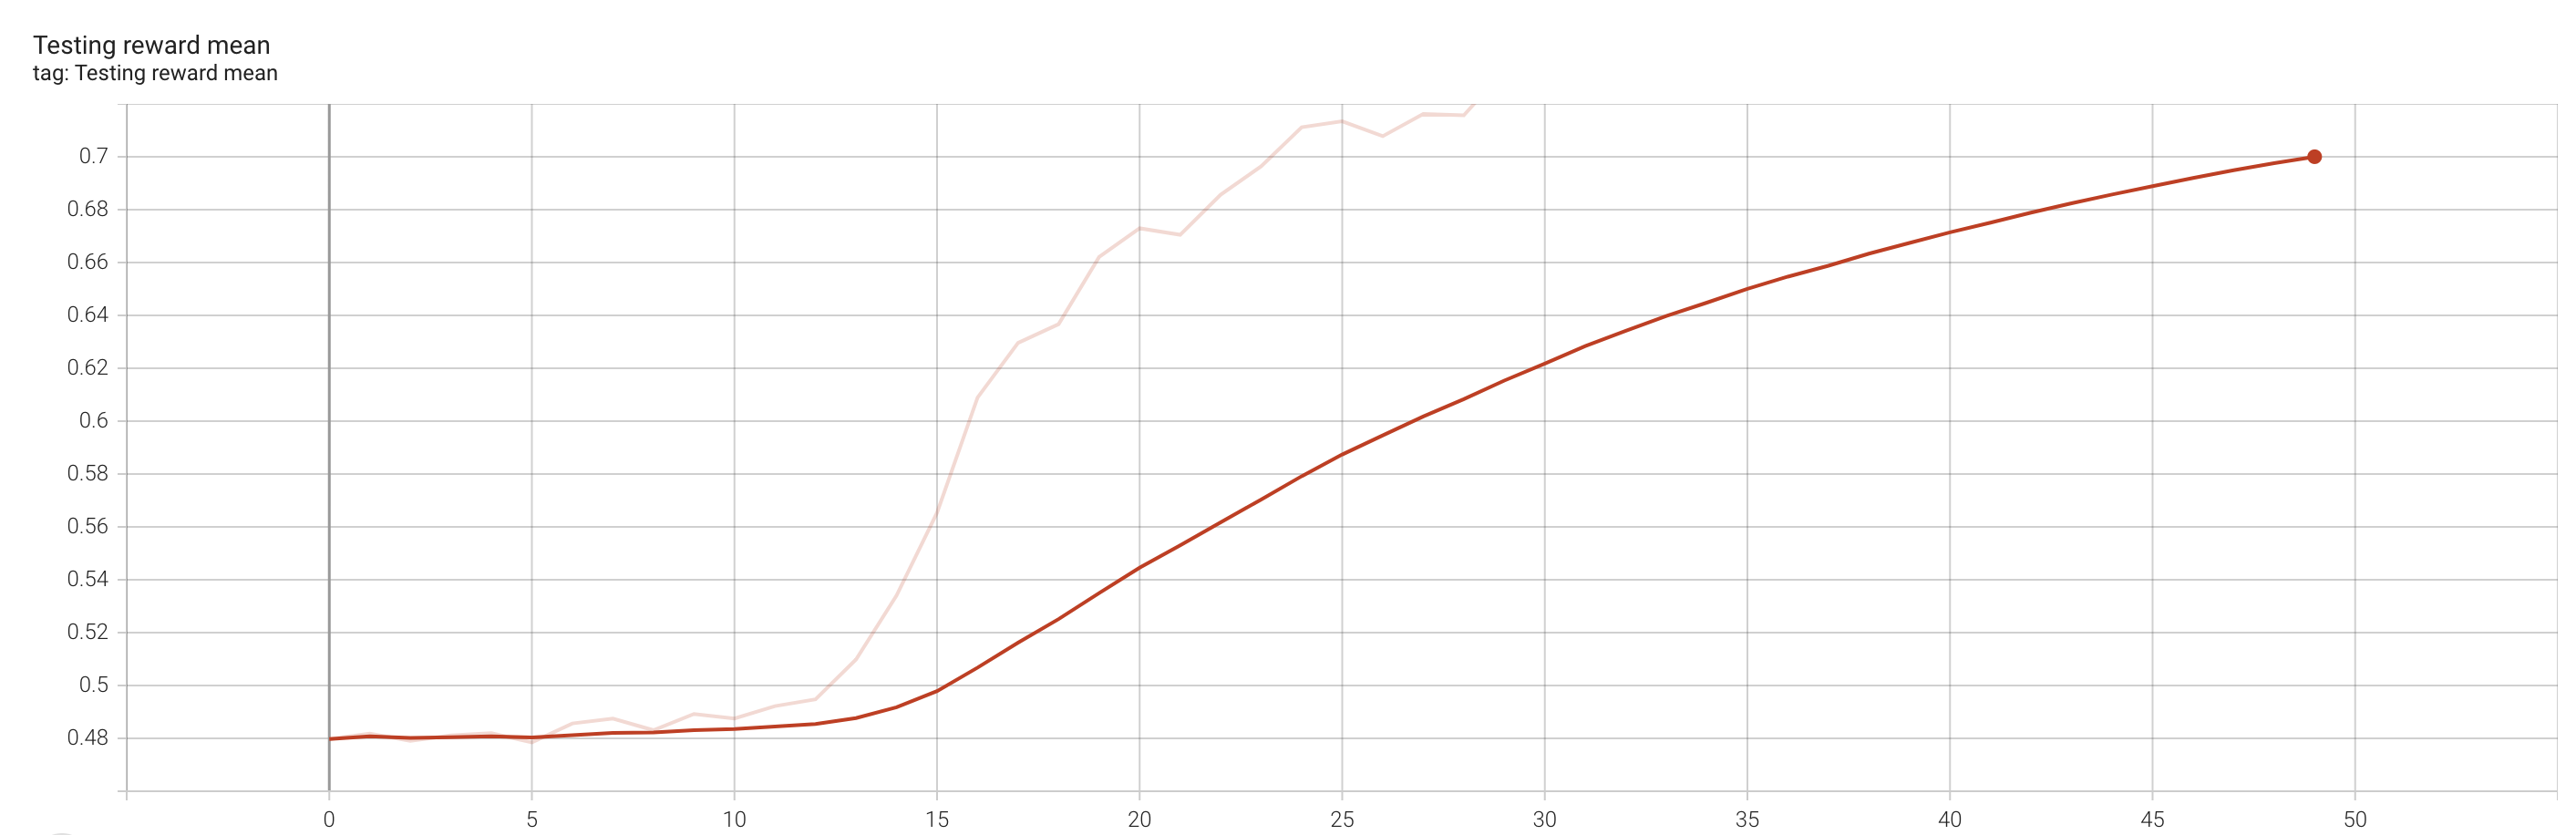
\includegraphics[width=1\textwidth]{figuras/experiments/policy_gradient/policy_gradient_normalized_image_reward_50_epochs/testing_reward_mean.png}
	\caption[Experimento Actor Critic 3 - Testing reward mean]{Experimento Actor Critic 3 - Testing reward mean}
	\label{fig-experimento-actor-critic-3-testing-reward-mean}
\end{figure}
\begin{figure}[H]
	\centering
	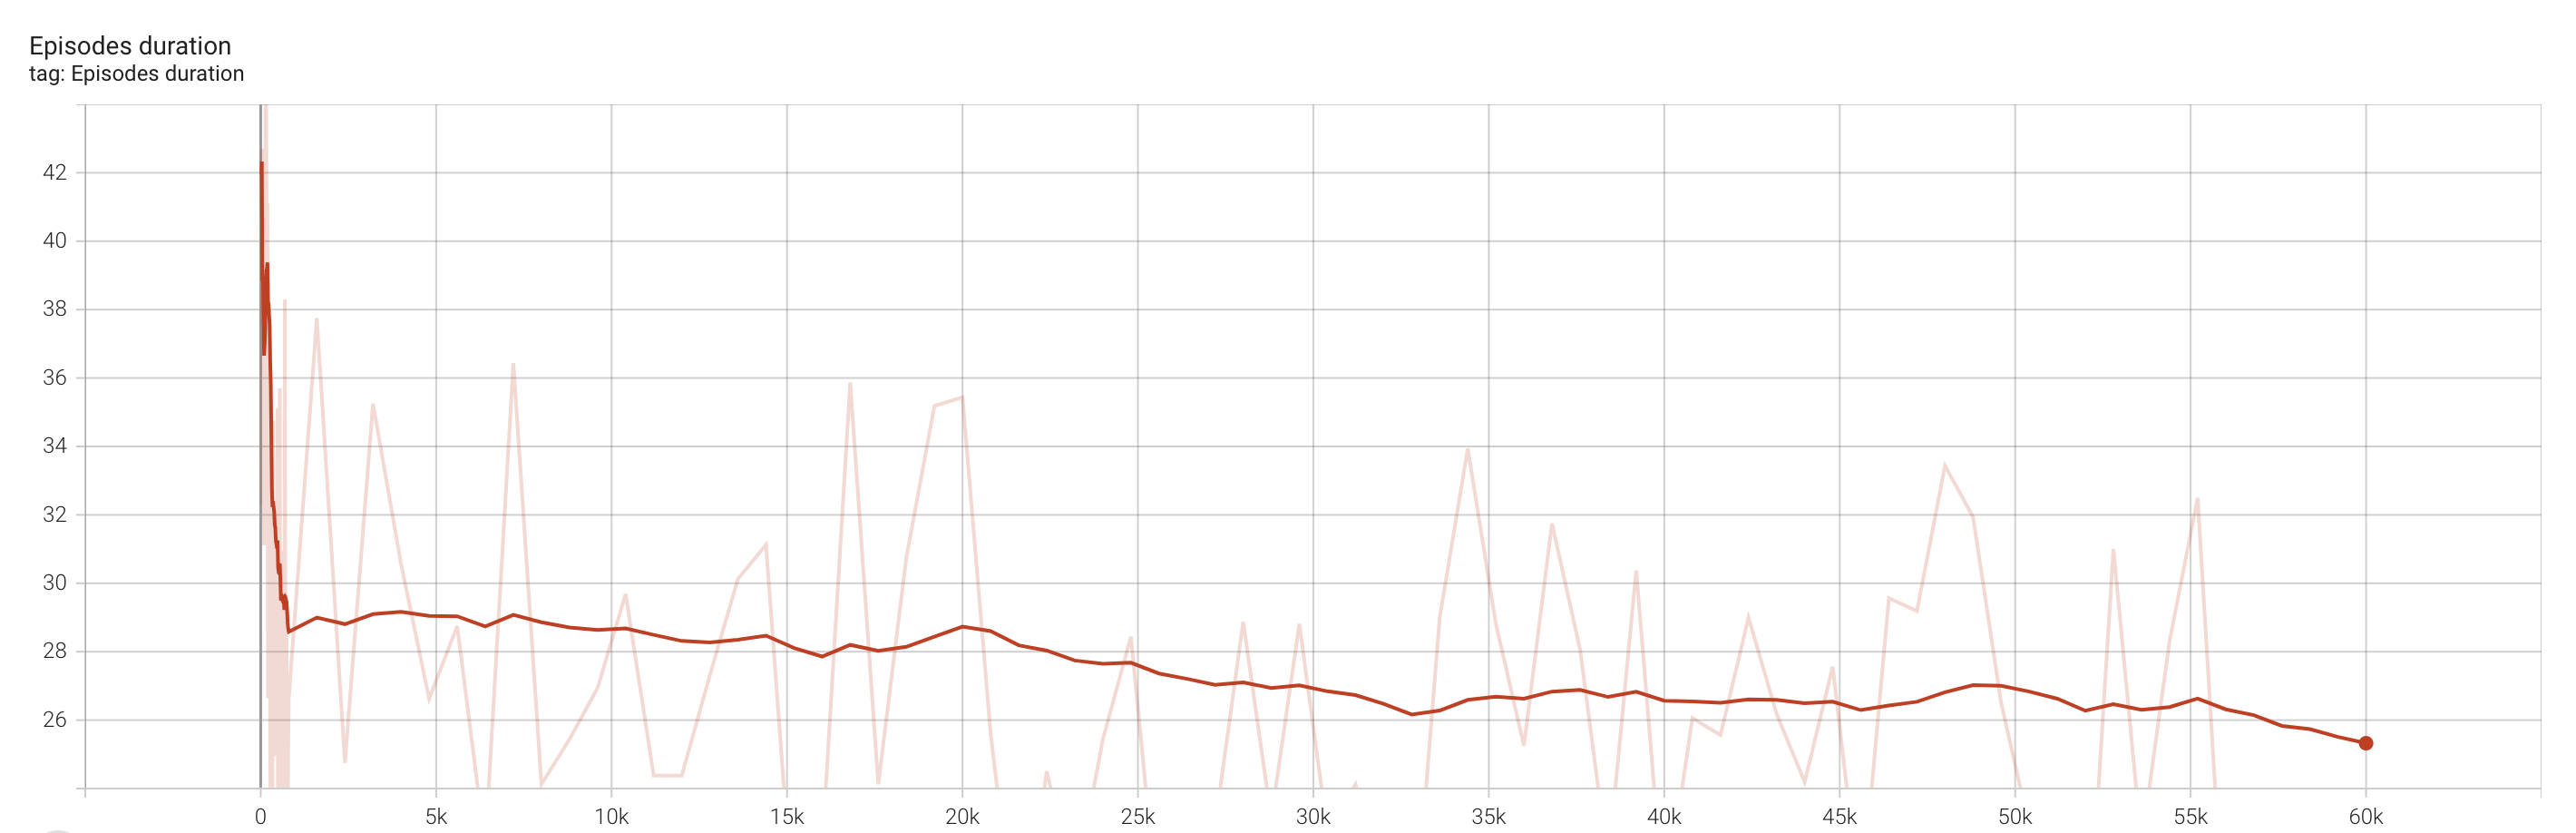
\includegraphics[width=1\textwidth]{figuras/experiments/policy_gradient/policy_gradient_normalized_image_reward_50_epochs/episodes_duration.png}
	\caption[Experimento Actor Critic 3 - Episodes duration]{Experimento Actor Critic 3 - Episodes duration}
	\label{fig-experimento-actor-critic-3-episodes-duration}
\end{figure}

\section{Vision Transformers}
\label{resultados-vision-transformers}

\begin{figure}[H]
	\centering
	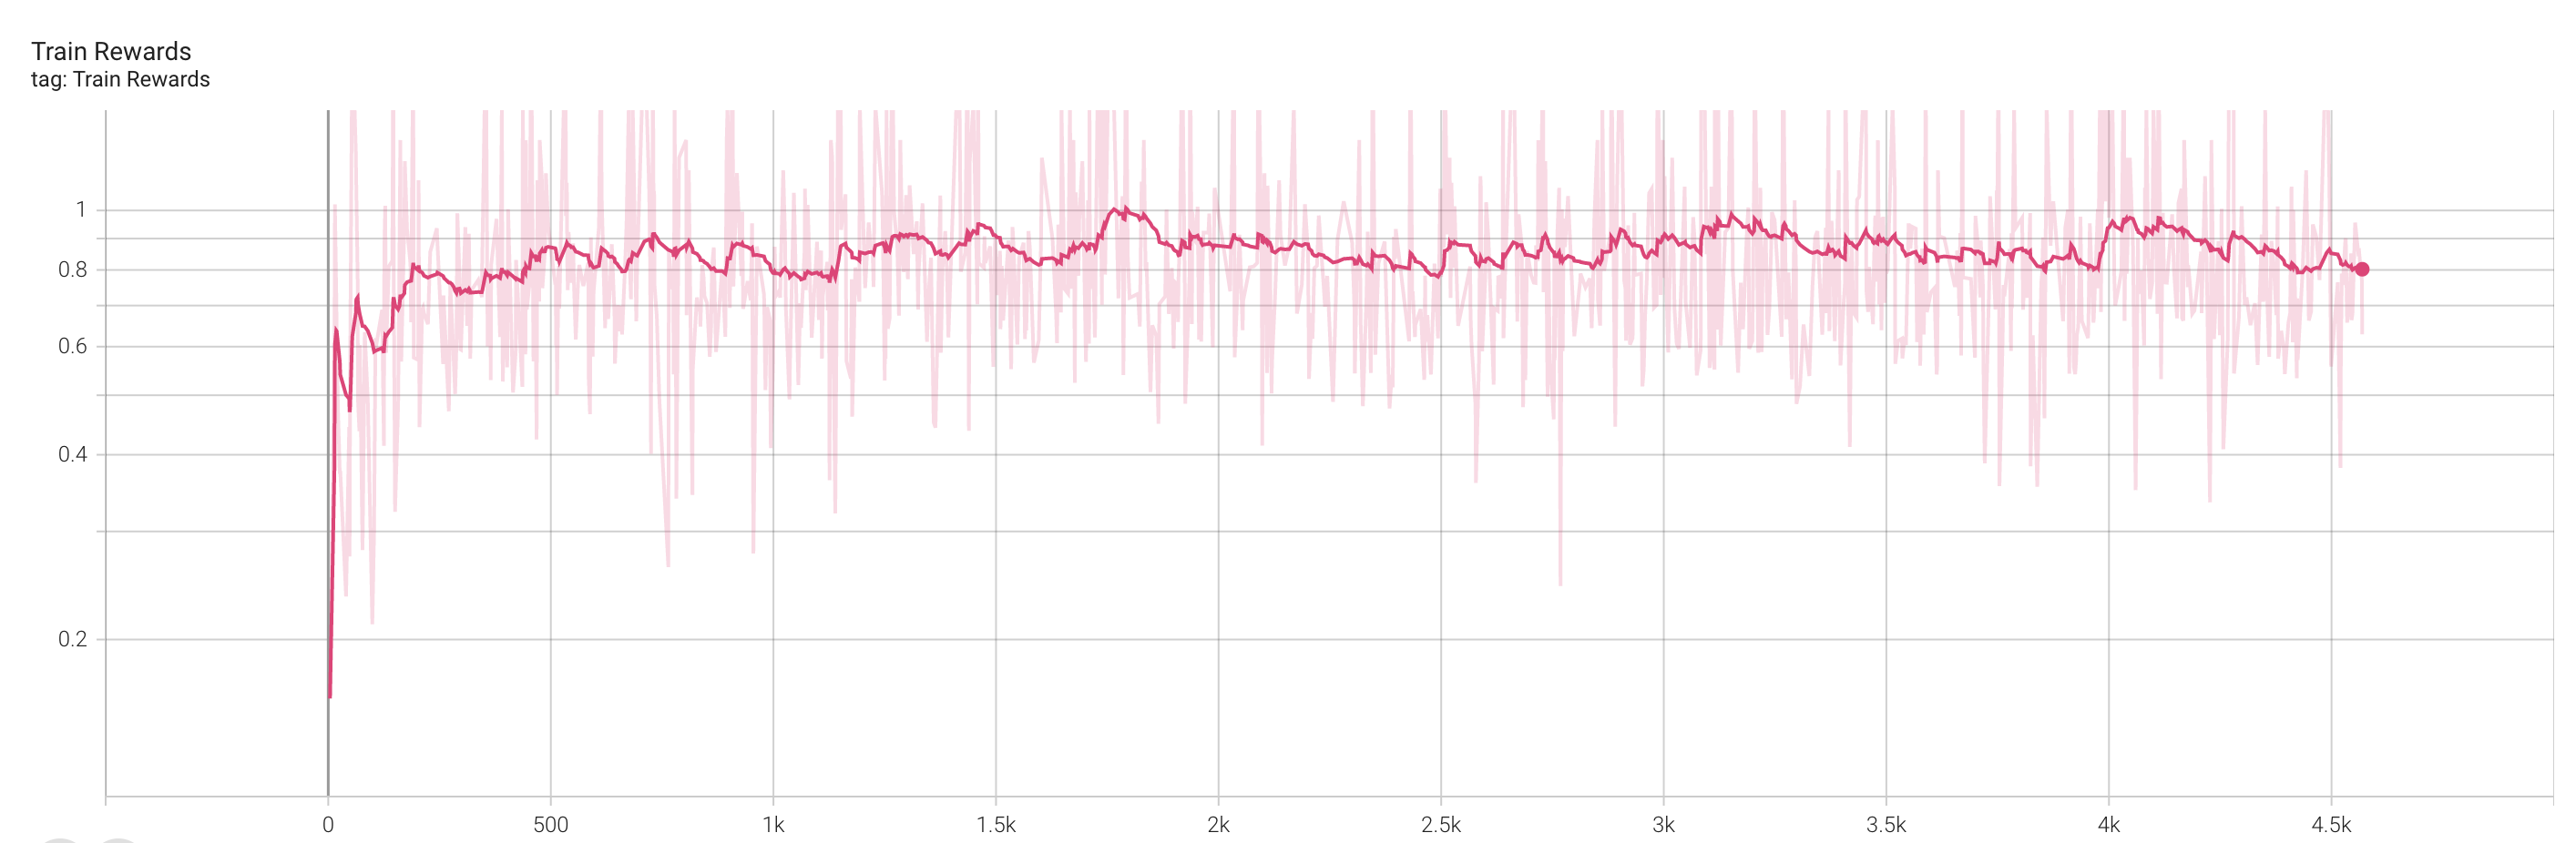
\includegraphics[width=1\textwidth]{figuras/experiments/vision transformers/train_rewards.png}
	\caption[Experimento \textit{Vision Transformer} - Training Reward Mean]{Experimento \textit{Vision Transformer} - Training Reward Mean}
	\label{fig-experimento-vision-transformer-1-training-reward-mean}
\end{figure}
\begin{figure}[H]
	\centering
	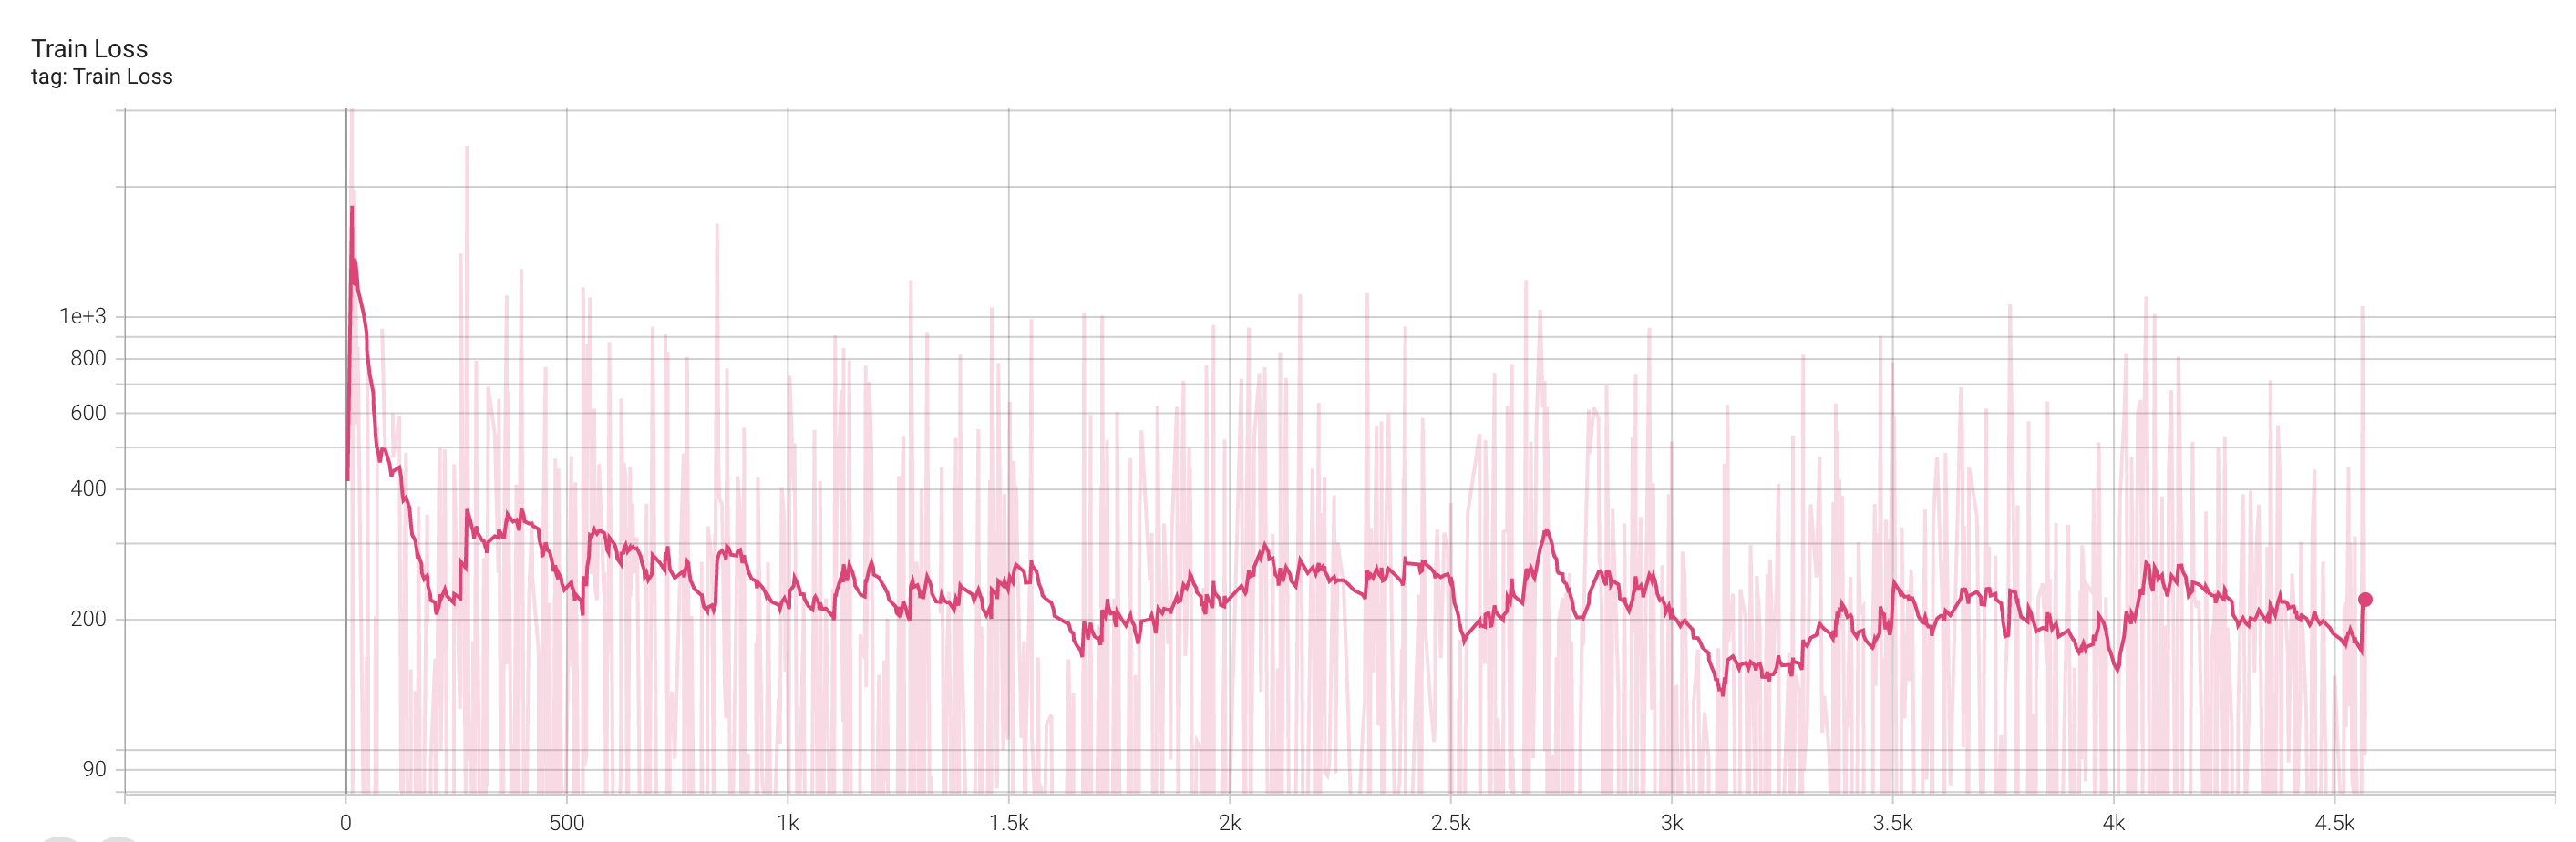
\includegraphics[width=1\textwidth]{figuras/experiments/vision transformers/train_loss.png}
	\caption[Experimento \textit{Vision Transformer} - Training Loss]{Experimento \textit{Vision Transformer} - Training Loss}
	\label{fig-experimento-vision-transformer-1-training-loss}
\end{figure}
\begin{figure}[H]
	\centering
	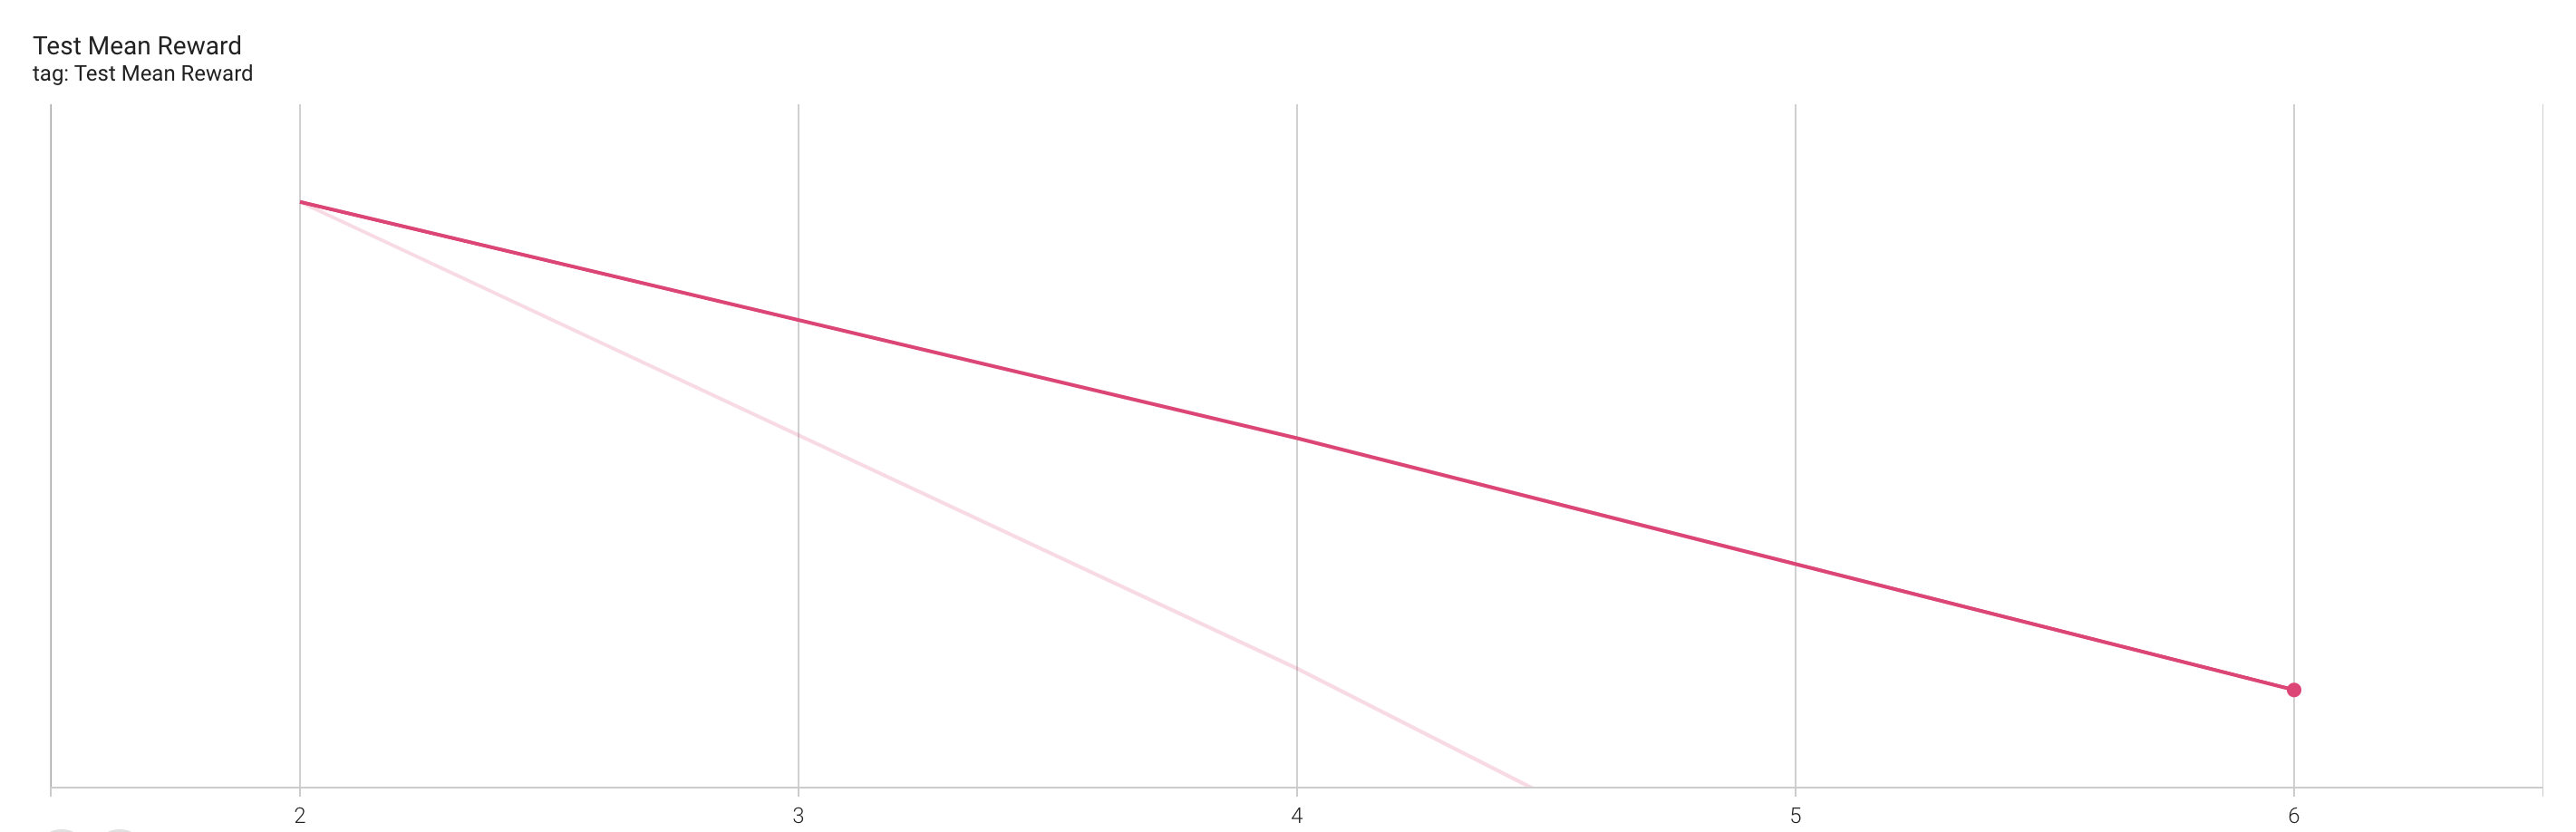
\includegraphics[width=1\textwidth]{figuras/experiments/vision transformers/test_mean_reward.png}
	\caption[Experimento \textit{Vision Transformer} - Testing reward mean]{Experimento \textit{Vision Transformer} - Testing reward mean}
	\label{fig-experimento-vision-transformer-1-testing-reward-mean}
\end{figure}
\begin{figure}[H]
	\centering
	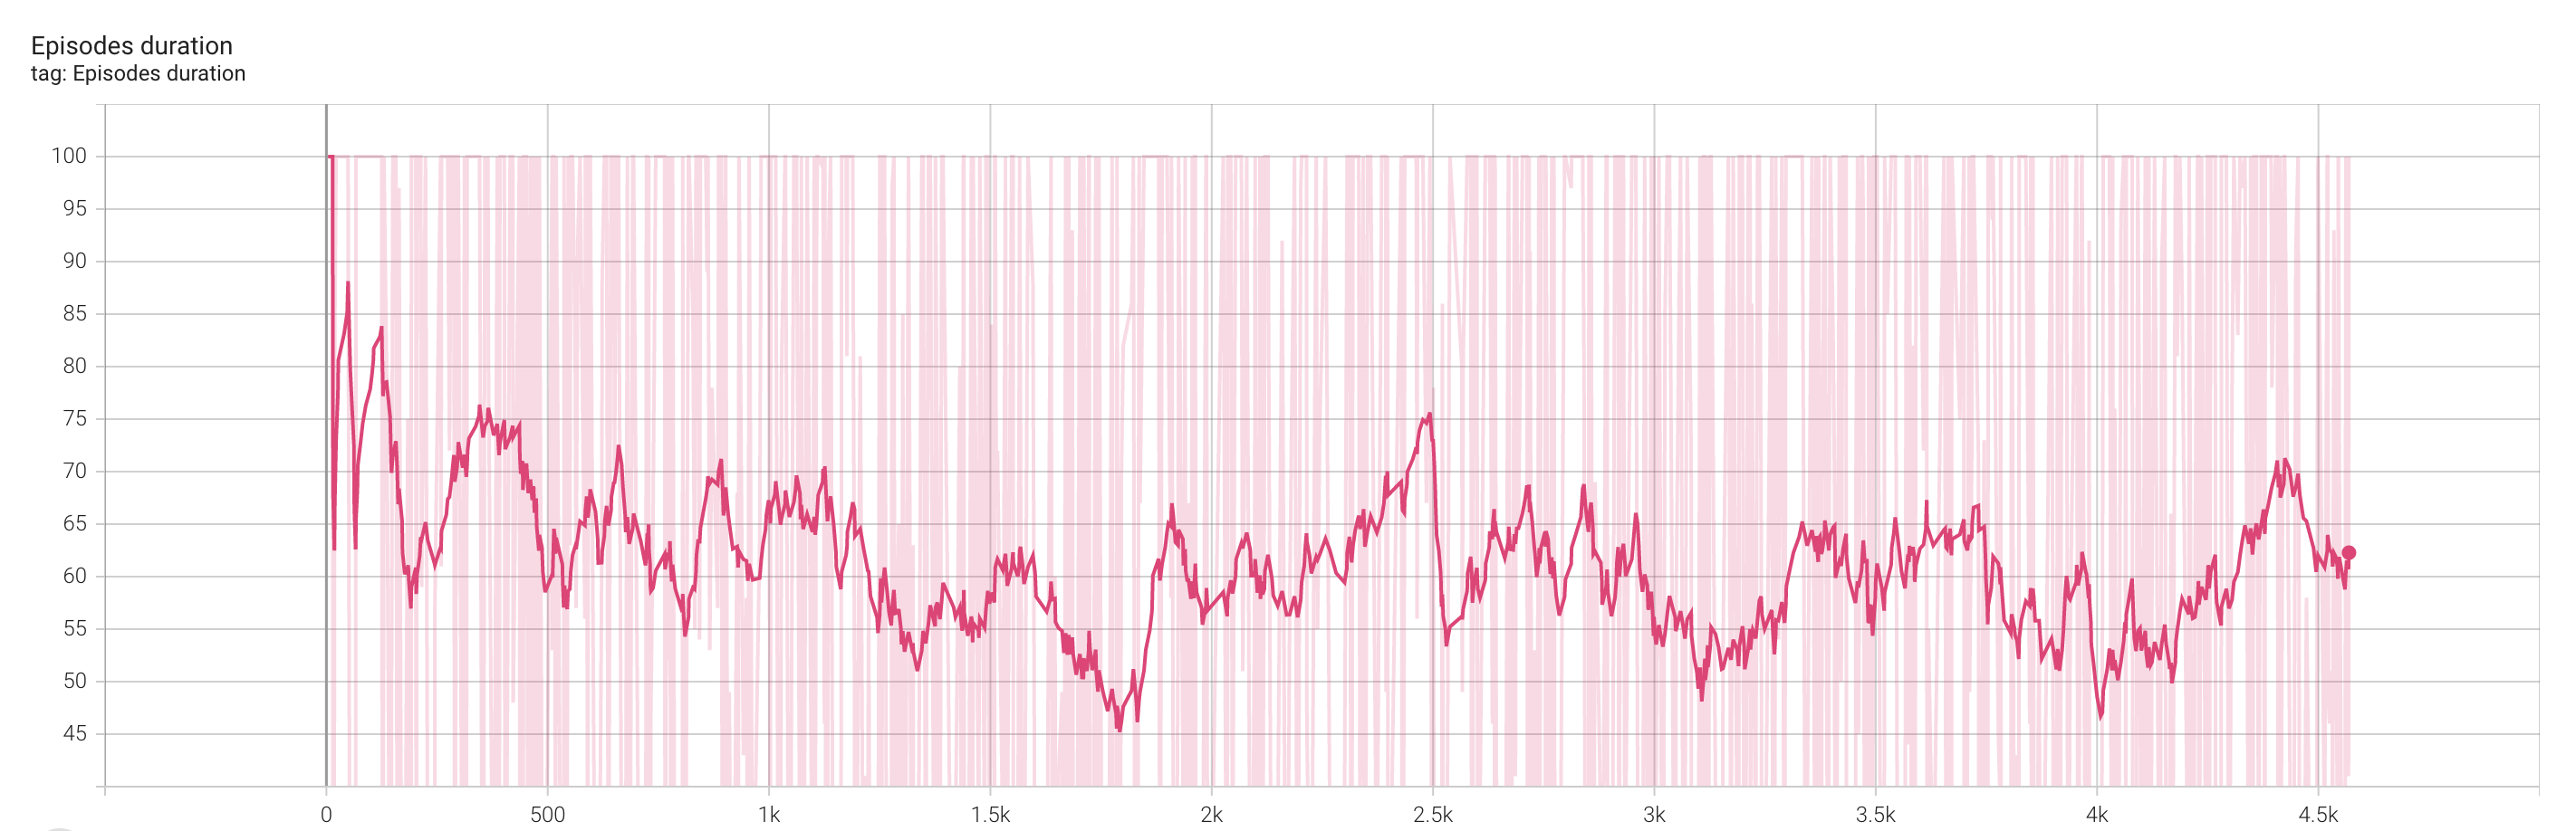
\includegraphics[width=1\textwidth]{figuras/experiments/vision transformers/episodes_duration.png}
	\caption[Experimento \textit{Vision Transformer} - Episodes duration]{Experimento \textit{Vision Transformer} - Episodes duration}
	\label{fig-experimento-vision-transformer-1-episodes-duration}
\end{figure}